\documentclass{llncs}

\usepackage{hyperref}
\usepackage{color}
%\usepackage[usenames,dvipsnames,table]{xcolor}
%\usepackage{colortbl}
\usepackage[usenames,dvipsnames]{xcolor}
\usepackage{listings, multicol}	
\usepackage{enumerate}
\usepackage{layouts}
\usepackage{times}
\usepackage{natbib}
\usepackage{notoccite}
\usepackage{todonotes}
%\usepackage{array}
\usepackage{alltt}
\usepackage{url}
\usepackage{amsmath}
\usepackage{amsfonts}
\usepackage{caption}
\usepackage{paralist}
\usepackage{soul}
\usepackage{enumitem}
\usepackage{appendix}

\usepackage{fancyhdr}
\usepackage{datetime}

\fancyhf{}
%\fancyfoot[L]{\today\ \currenttime}
\fancyfoot[C]{\thepage}
\pagestyle{fancy}

\let\proof\relax 
\let\endproof\relax
\usepackage{amsthm}

\usepackage{xspace}
\usepackage{tikz}
%\usepackage{cite}
\usepackage{subcaption}
\usepackage{calc}
\usetikzlibrary{calc}

\usepackage{fancyvrb}

\theoremstyle{definition}
%\newtheorem{definition}{Definition}[section]
\newcommand{\triple}[1]{\ensuremath{\langle #1 \rangle}}
\newcommand{\pair}[1]{\ensuremath{\left(#1\right)}}
\newcommand{\graph}[1]{\ensuremath{\mathcal{#1}}}
\newcommand{\graphset}[1]{\ensuremath{\mathbb{#1}}}

\newcommand{\sergey}[1]{\textcolor{magenta}{\marginpar{\sc Sergey} #1}}
\newcommand{\matthias}[1]{\textcolor{blue}{\marginpar{\sc Matthias} #1}}
\newcommand{\Qone}{$\boldsymbol{Q_1}$\xspace}
\newcommand{\Qtwo}{$\boldsymbol{Q_2}$\xspace}
\newcommand{\Qthree}{$\boldsymbol{Q_3}$\xspace}
\newcommand{\NP}{\ensuremath{\mathbf{NP}}}
\newcommand{\coNP}{\ensuremath{\mathbf{coNP}}}
\newcommand{\QBF}{\ensuremath{\mathbf{QBF}}}
\newcommand{\theory}{\ensuremath{\mathcal{T}}}

%\renewenvironment{tabular}{\oldtabular}{\endoldtabular}
%\renewcommand{\hline}{\oldhline}

\lstdefinestyle{model}{
  mathescape,
  columns=fullflexible,
  numbers=left,
  frame=single,
  escapechar=@,
  %escapeinside={(*@}{@*)}
  basicstyle=\scriptsize\ttfamily
}

\lstset{basicstyle=\small\ttfamily,breaklines=true}
\lstdefinestyle{small}{
  basicstyle=\scriptsize\ttfamily,
  breaklines=true
}

% redefine \VerbatimInput
\RecustomVerbatimCommand{\VerbatimInput}{VerbatimInput}%
{fontsize=\footnotesize,
   %
  frame=lines,  % top and bottom rule only
  framesep=2em, % separation between frame and text
  rulecolor=\color{Gray},
      %
  label=\fbox{\color{Black}proB encoding},
  labelposition=topline,
        %
% commandchars=\|\(\), % escape character and argument delimiters for
                              % commands within the verbatim
% commentchar=*        % comment character
}


\author{Matthias van der Hallen\dag
\thanks{Matthias van der Hallen is supported by a Ph.D. fellowship from the Research Foundation - Flanders (FWO - Vlaanderen).\vspace{-3em}}
, Sergey Paramonov\dag, Michael Leuschel\ddag, Gerda Janssens\dag}
\title{Knowledge Representation Analysis of Graph Mining}
\institute{\dag KU Leuven, \ddag Heinrich-Heine-Universit\"at D\"usseldorf}

\begin{document}
\maketitle
\begin{abstract}
%Many problems are inherently higher order due to their complex nature and composite structure.
Many problems, especially those with a composite structure, can naturally be expressed in higher order logic. %, for example due to their composite nature.
From a KR perspective modeling these problems in an intuitive way is a challenging task.
In this paper we study the graph mining problem as an example of a higher order problem. 
In short, this problem asks us to find a graph that frequently occurs as a subgraph among a set of example graphs.
We start from the problem's mathematical definition 
%which is clearly higher order 
to solve it
%the graph mining problem 
in three state-of-the-art specification systems.
%, IDP, ASP and ProB.
For IDP and ASP, which have no
native support for higher order logic, we propose the use of encoding
techniques such as the disjoint union technique and the saturation technique.
%The model in 
ProB
%, a formal specification language, 
benefits
from the higher order support for sets.
We compare the performance of the three approaches to get an idea of
the overhead of the higher order support.

%From a KR modeling perspective, we identify a number of desirable
%properties and discuss how the three approaches deal with them.
We propose higher-order language extensions for IDP-like
specification languages
and  discuss what kind of solver support is needed.
Native higher order shifts the burden of rewriting specifications using encoding techniques from the user to the solver itself.
%Many problems are inherently higher order due to their complex nature and composite structure.
%Modeling these problems in an intu\"itive way becomes a challenging task.
%This paper analyses, from a KR perspective, what difficulties arise when modeling such a problem, using the graph mining problem as an application-based example.
%We summarize several techniques such as the disjoint union technique or the saturation technique, and show how they can be applied to tackle the difficulties of modeling higher order problems, although it comes with a considerable loss of declarativeness and clarity of the specification.

%Furthermore, we identify several properties which should hold for a good modeling of the graph mining problem, from a KR perspective, and evaluate working models in several KR languages (IDP, ASP, ProB) on these properties.
%We also propose a ``faithfull'' encoding, which closely follows the mathematical definition of the graph mining problem and satisfies all different desired properties.
%Based on this faithfull encoding, we propose solver extensions that would shift the burden of rewriting the specification using the identified encoding techniques from the user to the solver itself, or would eliminate the need entirely.

%This paper analyses how problems of a composite and complex nature 
\end{abstract}

% !TEX root = notes.tex
\section{Introduction}
\todo{Add references and a discussion of higher-order systems such as DLVHEX, HiLog, Alloy*}
Many real world problems exhibit a composite structure consisting of multiple smaller problems which can be combined in many different configurations.
These types of problems lend themselves for a declarative approach as knowledge representations offers a transparent, natural and extendable model satisfying `The Principle of Elaboration Tolerance'~\citep{elaboration_tolerance}.
Delarative programming distinguishes itself by the ease with which declarative specifications can be adapted to variations in which subproblems are used, and in the way they are combined.

Conversely, the smaller problems in these composite structures are often already NP or coNP complete.
Combining these already complex problems often raises the computational complexity of the composite problem, up to a level where it cannot be expressed using first order logic.
These problems become inherently higher order logic: We study the \emph{Graph Mining} problem as an example problem featuring such a raise in complexity.

Specification languages with support for higher oder logic exist, with different levels of support.
On the one hand, meta-programming, as known from Logic Programming~\citep{Abramson and Rogers 1989}, has inspired the introduction of higher-order atoms in DLVHex~\citep{?}  and the higher-order syntax in HiLog~\citep{?}.
As in Prolog, predicate symbols can be either constants (first-order case) or variables (second-oder case).
In the case of predicate variable symbols, these variables range over predicate names, and not the predicate space itself, essentially combining second-order syntax with first-order semantics. 
This is not enough to model the graph mining problem.

On the other hand, specification languages such as Alloy~\citep{?}, B~\citep{?}, TLA~\citep{?}, VDM~\citep{?} and Z~\citep{?}, that support state-based and machine-based formal methods typically extend predicate logic with sets and operators from relational algebra, offering higher order semantics.
ProB~\citep{?} is such a well-know system for Event-B.
%This level of support for higher-order logic is enough to model the graph mining problem.
We can express the graph mining problem in these languages directly using higher order, but in general these systems miss the flexibility to perform multiple different inferences such as model expansion and optimization without modifying the specification.
Furthermore, while some of these systems can express inductive definitions using either its completion or using a built-in transitive closure operator, this comes with a significant loss of readability.
Lastly, many of these systems are built directly on CP techniques and finite domain solvers, and consequently do not implement the recent revolutions in solving techniques such as CDCL.

For these reasons, we also look at specification languages that do not allow higher order syntax.
Examples of such languages are the IDP language and the ASP language.
For these languages, several techniques exist that allow the user to simulate higher order logic to model problems such as graph mining, potentially offering better performance than systems that allow higher order logic directly.

%We study the \emph{Graph Mining} problem as an example problem of such a raise in complexity, and detail some of the techniques that can be used to handle this.
%This includes the generalization of ad-hoc techniques as well as the combination of techniques from different logics.

Graph mining is a specific kind of \emph{frequent pattern mining}, 
%which is one of the ``super-problems'' in Data Mining.~\citep{?}
%In its basic form it is }
the task of enumerating patterns which occur frequently in a dataset.
A first class of \emph{pattern mining} is \emph{unstructured mining}, such as \emph{itemset mining}, where the pattern is a set of items without any additional structural relation between the different items. 
Because it does not require any structure, the \emph{unstructured mining} task does not compose multiple smaller problems.
Therefore the rise in computational complexity associated with problem composition does not occur and the problem is even of propositional nature.
\citet{tias_original} have demonstrated how the \emph{itemset mining} problem can successfully be modeled in a declarative way using CP techniques.

In recent years, focus has shifted from unstructured mining towards structured mining, such as graph or sequence mining.
Here, the items being mined exhibit additional structure, for example the edge relation in the case of graph mining, or the order of elements in a sequence.
%Graph mining has many applications; it is for example often used as a preprocessing step for machine learning algorithms}~\citep{pattern_mining_classification.
%\todo{This could easily be dropped, but for example Michael immediately asks the question 'where is graph mining used'}
The additional structure required by the graph mining problem introduces subproblems within the graph mining problem: We need to specify when a graph occurs within other graphs, leading to the concept of homomorphism checks.
%\Likewise, \matthias{(also due to the additional structure)}, we need to represent the objects in the graph mining problem in a way that makes it non-obvious to say whether two objects are identical, which gives rise to subgraph isomorphism detection.
Many different interpretations can be given to 
%these two problems
%\matthias{homomorphism checks and isomorphism detection}~
this problem\citep{subtree_overview}, and in general these variations of the homomorphism 
%\st{and isomorphism concepts }
concept
are NP-complete~\citep{}\matthias{referenties op te zoeken}.
While this gives rise to many wildly different algorithms in imperative languages~\citep{gspan,theta_subsumption}, these variations can be specified with only minimal changes using a declarative modelling approach.

In our case study of the graph mining problem, we start with from the mathematical model of graph mining, which is inherently higher order, and identify the following contributions:
\begin{compactitem}
\item We identify the higher order aspects of the graph mining problem and show how the problem can be modeled in IDP (which supports Existential Second Order and inductive definitions) in ASP ($\Sigma_{2}^{p}$), and in ProB (which supports higher order sets), proposing concrete modelling techniques such as the disjoint union technique. 
We also identify a set of desirable properties for a declarative encoding of the graph mining problem.
We compare how the different solutions perform, both with respect to the desirable properties as to computation time.
%\item We propose higher order language constructs for IDP and ProB extensions which greatly improve the ease of expressing the graph mining and other higher order problems.
%\item We indicate how to shift the burden of addressing the higher order aspects of the problem from modeler to the solver. 
\item We propose an encoding that closely follows the mathematical model of graph mining, and satisfies all desirable properties of a graph mining model.
We indicate how to shift the burden of addressing the higher order aspects of the problem using encoding techniques from modeler to the solver. 
Concretely, solver support is needed to translate the proposed higher order language constructs from the previous item to first order using e.g the disjoint union modeling technique.
We indicate how additional solver support can leverage these expressive constructs to work more efficient.
\end{compactitem}
%\todo{rewrite contributions to two points}
The paper is structured as follows: Section \ref{sec:formalization} introduces the formalization of graph mining, Section \ref{sec:modeling} introduces a logical model and discusses the primitives at the core of graph mining problem.
Then, Section \ref{sec:code} introduces graph mining encodings in IDP, ASP and ProB. Section \ref{sec:extension} discusses language extensions.
Section \ref{sec:related_work} discusses related work. Section \ref{sec:conclusion} draws conclusions and outlines possible future research directions.
%\section{Introduction}
Frequent Pattern Mining, one of the ``super-problems'' in Data Mining, has received significant attention over the last years \citep{pattern_mining_book}. Pattern mining in its basic form is the task of enumerating patterns which occur frequently in a dataset.
A first class of pattern mining is \emph{unstructured} mining, such as itemset mining, where the pattern is a set of items without any additional structural relation between the different items.
This problem, in nature, is propositional.
\citet{tias_original} have demonstrated how the \emph{itemset mining} problem can successfully be modeled in a declarative way using CP techniques.

In recent years, focus has shifted from unstructured mining towards structured mining, such as graph or sequence mining.
Here, the items being mined exhibit additional structure, for example the edge relation in the case of graph mining, or the order of elements in a sequence. Graph mining has many applications and one of them is the preprocessing step for the machine learning algorithms. Machine learning algorithms are designed to work with numeric data and cannot handle relational data natively. Graph mining is used to transform graph data into a numeric representation suitable for the learning algorithms~\citep{pattern_mining_classification}. Many variations of the graph mining problems exist \citep{subtree_overview} and many algorithms have been developed \citep{gspan,theta_subsumption}.

Recently, the declarative approach has been applied to unstructured mining. It has been a remarkable success: declarative models outperform all existing systems in terms of flexibility and expressivity. Initially, there was a significant gap in the runtime performance between specialized algorithms and the CP formulation \citep{tias_original,mining_cp_extra}, however, the gap has been filled with the more developed systems such as MiningZinc \citep{tias_declarative_pattern_mining}. 
This suggests to apply declarative techniques to structured mining and graph mining in particular. This direction of research just started getting attention in the declarative modeling community \citep{cp_sequence_mining,ilp_graph_mining}. 

From a knowledge representation and modeling point of view the problem of graph mining is way more complex and challenging than unstructured mining. 
To indicate why the problem is more complex, let us informally introduce the problem. We need to enumerate all graphs, called \textit{patterns}, that often enough \textit{occur} in the positively labeled example graphs and not too often in the negatively labeled.
Here, the meaning of \textit{occuring} corresponds to the pattern somehow \emph{matching} the example graph, for example, by the existence of a homomorphism or isomorphism.
For most of the variations of graph mining, checking whether there exists even a single matching is already \textit{NP}-complete \citep{subtree_overview}, which implies that not matching is \textit{CoNP}-complete. 
Furthermore, each pattern must be a connected graph, therefore the concept of inductive definitions must be present in the language.
% and only briefly slices the surface of complexity exhibited by the problem.

Structured mining is not only more complex and challenging than unstructured mining, it also benefits even more from a declarative approach.
Here, knowledge representation offers a transparent, natural and extendable model satisfying The Principle of Elaboration Tolerance \citep{elaboration_tolerance}, where a variant of a problem can be modeled by adding or removing a constraint.
For example, the differences between the different ways of matching as mentioned above lead to minimal changes in the model.

Our main goal is to investigate the problem of graph mining using the KB-approach~\ref{} from knowledge representation and reasoning. 
We start with from the mathematical model of graph mining, which is inherently higher order, and identify the following contributions:

\begin{itemize}
\item We identify the higher order aspects of the graph mining problem and show how the problem can be modeled in IDP (which supports Existential Second Order and inductive definitions) and in ProB (which supports higher order sets).
\item We propose higher order language constructs for IDP and ProB extensions which greatly improve the ease of expressing the graph mining and other higher order problems.
\item We indicate how to shift the burden of addressing the higher order aspects of the problem from modeler to the solver. 
Concretely, solver support is needed to translate the proposed higher order language constructs from the previous item to first order using e.g the disjoint union modeling technique.
We indicate how additional solver support can leverage these expressive constructs to work more efficient.
\end{itemize}

The paper is structured as follows: Section \ref{sec:formalization} introduces the formalization of graph mining, Section \ref{sec:modeling} introduces a logical model and discusses the primitives at the core of graph mining problem.
Then, Section \ref{sec:code} introduces graph mining encodings in IDP, ASP and proB. Section \ref{sec:extension} discusses language extensions.
Section \ref{sec:related_work} discusses related work. Section \ref{sec:conclusion} draws conclusions and outlines possible future research directions.

\section{Formalization of the graph mining problem}\label{sec:formalization}
We start with a comprehensive formal definition of the graph mining problem.


\begin{definition}
A labeled graph \graph{G} is a triple $\triple{V,E,l}$ where $V$ is the set of vertices or nodes, $E$ is a binary predicate on $V$ that represents the set of edges and $l$ is a unary function from $V$ to a set of labels.
\end{definition}


\begin{definition}
A graph $\graph{G} = \triple{V,E,l}$ is \emph{connected} iff for each pair of vertices $v$ and $v'$ in $V$, there exists an edge $\pair{v,v'} \in E$ or there exists a sequence $v \ldots v_{1} \ldots v_{n} \ldots v'$ such that there exist edges $\pair{v,v_{1}}$, $\pair{v_{i},v_{i+1}}$ and $\pair{v_{n},v'} \in E$.
\end{definition}


\begin{definition}
A graph homomorphism $f$ from a labeled graph $\graph{G} = (V,E,l)$ to a labeled graph $\graph{G}' = (V',E',l')$ is an injective mapping f : $V \rightarrow V'$ from vertices of $\graph{G}$ to vertices of $\graph{G'}$ such that:
\begin{itemize}
\item $\forall u,v \in V, \pair{u,v} \in E \implies \pair{f(u),f(v)} \in E'$ (the mapping preserves edges), and 
\item $\forall v \in V : l(v) = l(f(v))$ (the mapping respects labelings).
\end{itemize}
If there exists such a graph homomorphism from graph $\graph{G}$ to $\graph{G'}$ we say $\graph{G}$ is \emph{homomorphic} with $\graph{G'}$.
\end{definition}

\begin{definition}
\label{def:GM1}
Given a pair $\triple{\graphset{E}_{+},\graphset{E}_{-}}$ consisting of a set of \emph{positive} and \emph{negative} examples of \emph{labeled graphs}, respectively,
\emph{Graph mining} is the problem of finding a \emph{connected labeled graph} $\graph{P}$, called a \emph{pattern},
that is \emph{homomorphic} with at least $N_{+}$ positive, while homomorphic with at most $N_{-}$ negative examples. We call these homomorpishms the positive (negative) homomorphisms, and the restriction on their number the positive (negative) homomorphic property, respectively.
\end{definition}

\begin{figure}[h]
  \centering
  \begin{subfigure}[b]{0.3\textwidth}
    \centering
    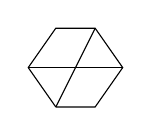
\begin{tikzpicture}[scale=.5]
      \draw (1,1) -- (2,1) -- (2.7,2) -- (2,3) -- (1,3) -- (0.3,2) -- (1,1);
      \draw (1,1) -- (2,3);
      \draw (2.7,2) -- (0.3,2);
    \end{tikzpicture}
    \caption{Positive Example\label{fig:pos}}
  \end{subfigure}
  ~
  \begin{subfigure}[b]{0.3\textwidth}
    \centering
    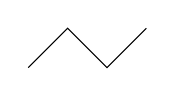
\begin{tikzpicture}[scale=.5]
      \coordinate (1) at (0,0);
      \coordinate (2) at (1,1);
      \coordinate (3) at (2,0);
      \coordinate (4) at (3,1);
      \draw (1) -- (2) -- (3) -- (4);
    \end{tikzpicture}
    \caption{Negative Example\label{fig:neg}}
  \end{subfigure}
  ~
  \begin{subfigure}[b]{0.3\textwidth}
    {
      \setcounter{subfigure}{0}
      \renewcommand\thesubfigure{\Roman{subfigure}}
      \centering
      \begin{subfigure}[b]{0.45\textwidth}
        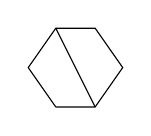
\begin{tikzpicture}[scale=.5]
          \draw (1,1) -- (2,1) -- (2.7,2) -- (2,3) -- (1,3) -- (0.3,2) -- (1,1);
          \draw (2,1) -- (1,3);
        \end{tikzpicture}
        \caption{Valid\label{fig:correctcandidate}}
      \end{subfigure}
      ~
      \begin{subfigure}[b]{0.45\textwidth}
        \begin{tikzpicture}[scale=.5]
          \draw (1,2) -- (2,3) -- (3,3);
        \end{tikzpicture}
        \caption{Invalid\label{fig:incorrectcandidate}}
      \end{subfigure}
    }
    \caption{Pattern Candidates\label{fig:candidates}}
  \end{subfigure}
  \caption{A graph mining instance ($N_{+}=1, N_{-}=0$) with pattern candidates.\label{fig:ex1}}
\end{figure}

%    \begin{tikzpicture}[scale=.5]
%        \coordinate (1) at (0,0);
%        \coordinate (2) at (1,1);
%        \coordinate (3) at (2,0);
%        \coordinate (4) at (3,1);
%        \draw (1) --
%              (2) --
%              (3) --
%              (4);
%    \end{tikzpicture}, ...

Take, for example, the problem set shown in Figure~\ref{fig:ex1}.
There is one positive example (Fig~\ref{fig:pos}), and one negative example (Fig~\ref{fig:neg}).
We assume all nodes have the same label.
Figure \ref{fig:candidates} shows a valid and an invalid pattern.
Requiring at least one homomorphism with a positive example, and allowing no homomorphisms with negative examples (i.e. problem parameters $N_{+}=1$ and $N_{-}=0$), Figure \ref{fig:correctcandidate} represents a valid pattern.
It is clear that there exists a mapping from each node from the valid pattern to a node of the positive example, while no such mapping exists for the negative example.
Looking at Figure \ref{fig:incorrectcandidate}, this graph is clearly homomorphic with both the positive as well as the negative example. Therefore, it is not a pattern.

\subsection{Canonical patterns}
To extend on the graph mining task described above, we can look for multiple patterns, instead of just one.
In this case, one can impose restrictions on the different patterns that are found.
For example, it stands to reason that one wants only \emph{canonical} solutions, meaning that no two patterns found are \emph{isomorphic}.

\begin{definition}
\label{def:isomorphism}
A graph isomorphism $f$ between two labeled graph $\graph{G} = \triple{V,E,l}$ and $\graph{G'} = \triple{V',E',l'}$ is a \emph{one-to-one} mapping $V \rightarrow V'$ 
such that $f$ represents a homomorphism from $\graph{G}$ to $\graph{G'}$,
and its inverse $f^{-1}$ represents a homomorphism from $\graph{G'}$ to $\graph{G}$.
If there exist such graph isomorphisms between $\graph{G}$ and $\graph{G'}$ we say $\graph{G}$ and $\graph{G'}$ are \emph{isomorphic}.
\end{definition}

We now can define the concept of a canonization and the related concept of a canonical graph. 
%Having defined the concept of a homomorphism, we want to define the concept of a \emph{canonical} graph.
To define this concept, we need to consider a multitude of graphs $\graph{G}$, each of which consists of a set of vertices $V$, an edge relation $E$ and a labeling function $l$. 
As the vertices themselves have no distinctive property, it is possible, and even beneficial to reuse the same, sufficiently large set of vertices $V$ for all example graphs as well as the mined patterns.

\begin{definition}
\label{def:canonicalForm}
Let $\graphset{G}$ be a set of graphs over a sufficiently large set of vertices $V$, closed under isomorphism.
A function $c$ for which $\forall \graph{G,H} \in \graphset{G} : \graph{G} \simeq \graph{H} \iff c(\graph{G}) = c(\graph{H})$ and $\forall \graph{G} \in \graphset{G} : \graph{G} \simeq c(\graph{G})$ hold, is called a \emph{canonization}.
The graph $c(\graph{G})$ is called the \emph{canonical form} w.r.t $c$, and is denoted by $\mathit{canon}(\graph{G})$.
\end{definition}

\begin{figure}[h]
  \centering
  \begin{subfigure}[b]{0.45\textwidth}
    \centering
    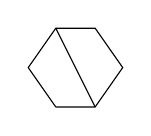
\begin{tikzpicture}[scale=.5]
      \draw (1,1) -- (2,1) -- (2.7,2) -- (2,3) -- (1,3) -- (0.3,2) -- (1,1);
      \draw (2,1) -- (1,3);
    \end{tikzpicture}
    \caption{First candidate pattern\label{fig:iso1}}
  \end{subfigure}
  ~
  \begin{subfigure}[b]{0.45\textwidth}
    \centering
    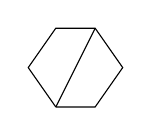
\begin{tikzpicture}[scale=.5]
      \draw (1,1) -- (2,1) -- (2.7,2) -- (2,3) -- (1,3) -- (0.3,2) -- (1,1);
      \draw (1,1) -- (2,3);
    \end{tikzpicture}
    \caption{Second candidate pattern\label{fig:iso2}}
  \end{subfigure}
  \caption{Possible patterns\label{fig:isomorphism}}
\end{figure}

Given the graph mining problem as specified in Figure~\ref{fig:ex1}, we have already established that Figure~\ref{fig:iso1} is a valid pattern.
When we try to mine a second pattern, we might suggest a pattern as shown in Figure~\ref{fig:iso2}.
A quick check, however, will show that there is a one-to-one mapping $f$ such that both $f$ as well as its inverse $f^{-1}$ preserve edges.
As a result, the first candidate pattern and the second are isomorphic.
By Definition~\ref{def:canonicalForm} only one of these two patterns can be the canonical form, and therefore only one of these two candidate patterns should be accepted as a valid pattern.

\subsection{Rewording}
%Given the mathematical definition of the graph mining problem above, w
We want to study how this formal mathematical definition can be expressed in the logics underlying the IDP~\cite{} and the ProB~\cite{} system.
First, we will reword the earlier definition~\textbf{Def.}~\ref{def:GM1} into an equivalent formal definition that uses logical sentences and language constructs available in general logics.
In doing this, it becomes evident that the graph mining problem has fundamental underlying characteristics that result in a higher order definition and specification.

%An attempt to model the Graph Mining problem in both IDP as well as ProB makes it clear
%that neither language allows us to express the problem to its full extent.
%We now try to link the shortcomings of each language to the expressiveness of the underlying logic on which they are built.

%First we introduce a new definition of the graph mining problem, equivalent to \textbf{Def.}~\ref{def:GM1}.
As mentioned above, the vertices in the graph mining problem have no distinctive property, and can be reused between different example graphs and patterns.
Therefore, we will assume one shared, sufficiently large set of vertices $V$ and represent example graphs over these vertices $V$ directly as a triple $\triple{Edge, Label, Class}$, consisting of an (binary) edge relation on $V$ and a labeling function over $V$, as well as a classification (positive/negative).

\begin{definition} \textbf{Graph Mining (redefined)}
\label{def:gm2}
Given a sufficiently large set of vertices $V$, and a set $\graphset{G}$ of graphs over this vertex set $V$, represented by $\triple{E, l, c}$ triples
where $E$ and $l$ represent the edge relation and labeling function over $V$ respectively,
%which consist of an edge relation, 
we look for a 
%(set $\graphset{P}$ of) \todo{cleanly extend this definition to multiple graphs, or separate the single and multiple pattern case again}
graph \graph{P} represented by tuple $\triple{E_{\graph{P}}, l_{\graph{P}}}$ such that:
%for at least $N_{+}$ of the triples $\triple{ E, l, C}$ with $C=Pos$, and for at most $N_{-}$ of such triples with $C=Neg$, there exists a function $f$ s.t. $\forall u,v \in V, \pair{u,v} \in E_{p} \implies \pair{f(u),f(v)} \in E$ and $\forall v \in V : l_{p}(v) = l(f(v))$.

\begin{itemize}
\item $\#\Big\lbrace \triple{E,l,pos} \in \graphset{G} \; | \; \exists f : \text{f is an homomorphism from \graph{P} to \triple{E,l,pos}} \Big\rbrace \geq N_{+}$

\item $\#\Big\lbrace \triple{E,l,neg} \in \graphset{G} \; | \; \exists f : \text{f is an homomorphism from \graph{P} to \triple{E,l,neg}} \Big\rbrace \leq N_{-}$
\end{itemize}
\end{definition}

\begin{definition} \textbf{Canonical Patterns}
A set of \emph{canonical patterns} is a set $\graphset{P}$ of graphs $\graph{P}_{i}$, such that for each pair of different elements(of \graphset{P}) $\graph{P}_{i}, \graph{P}_{j}$ holds that there does not exist an isomorphism between $\graph{P}_{i}$ and $\graph{P}_{j}$.
\end{definition}

As evidenced from the definitions above, graphs are the main concept in the graph mining problem, and, when represented using a triple $\triple{E,l,c}$, graphs are inherent \emph{higher order objects}.
A set of graphs, such as the argument of the cardinality operator above or the set of example graphs $\graphset{G}$, is equivalent to a set of triples.
The most straightforward representation of such a set would therefore be a ternary predicate.
As the domains of this predicate range over predicates and functions, this predicate would be a higher order predicate.

It is very natural to consider and represent each graph as a \emph{coherent} ensemble of its own components: all characteristics (edges, labeling \ldots) of a graph are represented by separate entities or concepts, which are grouped together for each graph $\graph{G}$ in the triple that describes it. We refer to this as the \emph{local coherence} of the graph representation.
Not only is this a very natural representation, this representation also makes it very explicit that all example graphs are \emph{independent}, and that the searches for homomorphisms between a pattern and example graphs are independent as well.
This motivates us to reason about graphs as locally coherent objects in our logical models as well.
However, the higher order representations needed to reason about graphs and sets of graphs as \emph{coherent} objects in our models are not yet fully supported by the logics of IDP and ProB.
In the following section we discuss how we can deal with this.

%When reasoning about graphs, we see \emph{each graph} as a \emph{coherent} ensemble of its own components: 
%all characteristics (edges, labeling \ldots) of a graph are represented by separate entities or concepts, which are grouped together for each graph $\graph{G}$ in the triple that describes it.
%We refer to this as the \emph{local coherence} of the graph representation.
%As graphs are the main concepts we talk about in the graph mining problem, keeping this concept together leads to a natural KR representation.
%Furthermore, this locally coherent representation makes it very explicit that all example graphs are \emph{independent}, and that the search for a homomorphism between pattern and example graph is independent as well.
%A good solver can then discover this independence and leverage it to achieve better performance.

%A set of graphs, such as the argument of the cardinality operator above or the set of example graphs $\graphset{G}$, is equivalent to a set of triples.
%The most straightforward representation of such a set would therefore be a ternary predicate.
%As the domains of this predicate range over predicates and functions, this predicate would be a higher order predicate.

%These higher order representations for graphs and sets of graphs are not yet fully supported by the logics of IDP and ProB.
%In the following section we discuss how we deal with them.
%\todo{Illustrate local coherence with table}


\section{Modeling}\label{sec:modeling}
In this section, we show how state-of-the-art KR systems without support for higher order, such as IDP and ASP, can model the graph mining problem and its higher order features using encoding techniques.
We identify the desirable properties that from a KR perspective should hold for a good modeling of the graph mining problem and we evaluate how a modeling in ProB, as a KR language with support for higher order sets, satisfies these properties.
%We conclude with a comparison of the performance of the three approaches. 

\subsection{IDP}
We assume some familiarity with the IDP system.
An extensive introduction can be found in~\cite{}.
\subsubsection{Existential Second Order}
The IDP language can express problems that consist of a set of symbols, called the vocabulary $V$, and a theory, called $T$, that uses symbols from this vocabulary.
The symbols in the vocabulary can be propositions, but they can also represent predicates and functions.
These last two types of symbols make the vocabulary, in general, a \emph{second order} object: it is an object that itself \emph{contains} not only propositional symbols, but also first order symbols.
For example, vocabulary V in Listing \ref{lst:vocabularyExample} is a second order vocabulary as it contains the first order symbol \lstinline{Edge/2}.

The theory $T$ is restricted to a \emph{first order} theory, extended with types, arithmetic, aggregates, and inductive definitions.
An example of such a theory is given in Listing \ref{lst:vocabularyExample}.
It contains an inductive definition for \lstinline{Path/2}, and one constraint.

Our inference of choice in the graph mining problem is model expansion; we search for an interpretation $I$ of symbols in the vocabulary $V$, called a \emph{model}, such that this interpretation $I$ satisfies the theory $T$.
This corresponds to the implicit \emph{existential quantification} of all symbols in the vocabulary, both the propositional as well as the first order symbols.
In the example of Listing~\ref{lst:vocabularyExample}, we expand the $S$ to the model $Result$ with 3 edges: One from the first node to itself, one from the first node to the second, and one from the second to the third.
Path contains all corresponding paths between these three nodes.

In conclusion, we say IDP can express model expansion for \emph{Existential Second Order} problems.
This level of expressiveness is not sufficient for general graph mining problems.
We will discuss the several issues in the remainder of this section.


\begin{lstlisting}[mathescape,style=model,caption=\ldots, label=lst:vocabularyExample]
vocabulary V{
    type Node
    Edge(Node, Node)
    Path(Node, Node)
}
theory T : V {
    $\forall$n[Node] : $\exists$n2[Node] : Edge(n,n2) $\lor$ Edge(n2,n).
    {
        Path(x,y) $\leftarrow$ Edge(x,y).
        Path(x,y) $\leftarrow \exists$z[Node] : Path(x,z) $\land$ Path(z,y).
        Path(x,y) $\leftarrow$ Path(y,z).
    }
}
structure S : V{
    Node = {1;2;3}
}

structure Result:V{
    Node = {1; 2; 3}
    Edge = {1,1; 1,2; 2,3}
    Path = {1,1; 1,2; 1,3; 2,1; 2,2; 2,3; 3,1; 3,2; 3,3 }
}
\end{lstlisting}


%problems in which there is an existentially quantified, generally second order, vocabulary of symbols and a first order theory with symbols from that vocabulary.
\paragraph{Issue 1}
First, we must represent the set of example graphs, as specified in \textbf{Def.}~\ref{def:gm2}. 
This definition uses a higher order predicate(See \textbf{Listing}~\ref{lst:HOPred}) \lstinline{GraphInst/3} with as first argument the edge predicate and as second argument the label function. For the first graph, \lstinline|{1,2; 2,1}| and \lstinline|{1\mapsto a; 2\mapsto b}| respectively. 
It represents a single graph as a tuple of predicates and functions, visualized in \textbf{fig.}~\ref{fig:LocalCoherence} as the solid shape.
It is clear that this representation is highly locally coherent, and preserves the independence of graph characteristics.
However, as we are restricted to \emph{Existential} Second Order, we cannot express this higher order predicate in IDP.

One possible solution is to replicate for each graph the different characteristic predicates and functions, as shown
in \textbf{Listing}~\ref{lst:multiglobal} and visualised as the dashed shapes in \textbf{Fig.}~\ref{fig:LocalCoherence}.
In this encoding, every graph has its own edge predicate and label function. 
Because there is now no relation between the different edge predicates and label functions, it is necessary to formulate our theory in terms of these different predicates and functions.
Encoding a property such as ``In every graph, all nodes have at least two outgoing edges'' must be stated for each of the edge predicates explicitly:
%duplicate in our theory the constraints and properties (i.e. homomorphism) about these example graphs and their relations as well: we cannot generalize over the names of these edge relations and labeling functions.
\begin{center}
\begin{tabular}{c}
\begin{lstlisting}[mathescape]
$\forall$ n[Node] : $\exists$ n1,n2[Node] : E1(n, n1) $\land$ E1(n,n2) $\land$ n1 $\neq$ n2.
$\forall$ n[Node] : $\exists$ n1,n2[Node] : E2(n, n1) $\land$ E2(n,n2) $\land$ n1 $\neq$ n2.
\end{lstlisting}
\end{tabular}
\end{center}

It is clear that this solution is undesirable due to the way it scales and the theory modifications needed with growing problem instances.
It retains the local coherence and independence of graph characteristics when it comes to data representation, but prohibits the abstraction (generalization) of knowledge in the theory.
% about these properties, as evidenced by our obligation to duplicate the theory for each graph.

%GraphInst(E:Node$\times$Node,Lb
\begin{center}
\begin{minipage}{0.68\linewidth}
\begin{lstlisting}[mathescape,caption=Higher order predicate modeling the set $\graphset{G}$ of Def~\ref{def:gm2}.,label=lst:HOPred]
GraphInst({1,2; 2,1},{1$\mapsto$a; 2$\mapsto$b},pos).
GraphInst({1,3; 2,1},{1$\mapsto$c; 2$\mapsto$b; 3$\mapsto$a},neg).
\end{lstlisting}
\end{minipage}
\end{center}

\begin{minipage}[t]{0.45\linewidth}
\begin{lstlisting}[mathescape,caption=Multiple individual global relations,label=lst:multiglobal]
E1(1,2). lb1(1)=a.
E1(2,1). lb1(2)=b.
E2(1,3). lb2(1)=c.
E2(2,1). lb2(2)=b.
         lb2(3)=a.
\end{lstlisting}
\end{minipage}
\begin{minipage}[t]{0.1\linewidth}
 ~
\end{minipage}
\begin{minipage}[t]{0.45\linewidth}
\begin{lstlisting}[mathescape,caption=Disjoint union using indexed global relations,label=lst:indexedglobal]
E(g1,1,2). lb(g1,1)=a.
E(g1,2,1). lb(g1,2)=b.
E(g2,1,3). lb(g2,1)=c.
E(g2,2,1). lb(g2,2)=b.
           lb(g2,3)=a.
\end{lstlisting}
\end{minipage}




A more workable solution is to represent each characteristic property, such as the edge relation, by a single global relation for all graphs, as shown in \textbf{Listing}~\ref{lst:indexedglobal} and by the dotted shape in \textbf{Fig.}~\ref{fig:LocalCoherence}.
This relation behaves the way it should for a specific graph instance based on an additional argument serving as an identifier for the graph of interest.
%This gives rise to a set $G$ of \emph{graph identifiers}, one for each example graph.
This global relation now corresponds to the \emph{disjoint} or \emph{tagged union} of the graphs' relations, where the tags are drawn from a set $G$ consisting of graph identifiers.
It is clear that this representation forces us to give up the local coherence of graph characteristics that was present in \textbf{Def.}~\ref{def:gm2}.
%Nu kunnen we kijken wat deze truuk doet met onze mogelijkheid om de abstraction van de theory uit te drukken. Normaal mwillen we dit zo schrijven. Hoewel we nu de generalisatie kunnen uitdrukken, verplicht de restrictie tot existentieel s..o ons om de homomorphic mapping functies te tot een globale property te promoveren, hoewel we feitelijk niet geinteresseerd zijn in de concrete mappings. om om te gaan met de afhankelijkheid van deze functies op de spec. vb grafen moeten we... die nu erg lijkt op skolemisation. theory

%Using this trick however, does not influence our ability to 
Now we can generalize over the different graphs, so that we can encode the property stated above as:
\begin{center}
\begin{minipage}{0.95\linewidth}
\begin{lstlisting}[mathescape]
$\forall$ gid[GraphId] : $\forall$ n[Node] : $\exists$ n1,n2[Node] : E(gid, n, n1) $\land$ E(gid, n,n2) $\land$ n1 $\neq$ n2.
\end{lstlisting}
\end{minipage}
\end{center}

%But can we now express the abstraction (generalization) of knowledge about these properties, such as the positive homomorphic property?
%to separate the constraint describing the positive homomorphic property, and the coint on its number of occurrences.
%This, from a KR point of view, 
%Furthermore, the restriction to ESO requires us 
%As an example, we illustrate this trick by showing on the expression of the positive homomorphic property, where it greatly resembles Skolemization.
%As evidenced in \textbf{Def.}~\ref{def:gm2}, normally one would express the positive homomorphic property by quantifying (counting) over all graphs, requiring the existence of a function with the correct properties.
%Using the disjoint union representation, we can quantify over the set $G$ of graph identifiers instead of over the actual graphs.
%Therefore, this representation allows us to express this property.

\begin{figure}[h]
\centering
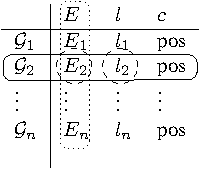
\includegraphics{CoherenceTable-crop.pdf}
\caption{Local coherence\label{fig:LocalCoherence}}
\end{figure}

%These three different ways of representing graphs are summarized in Fig~\ref{fig:LocalCoherence}.

\paragraph{Issue 2}
%Having solved\matthias{circumvented?} our first issue, 
Next, we would like to express the homomorphic property.
This can be done using a count aggregate, as shown in Listing~\ref{lst:QuantifyOutsideVocabulary}.
First we express the set of all example graphs to whom there exists a homomorphism from our pattern $\graph{P}$.
% generate the set of all example graphs to whom we can find a homomorphism from our pattern.
We do this by quantifying over all example graphs g or, per \textbf{issue 1}, their identifiers, and subsequently 
expressing the condition under which they are part of this set: i.e. that there must exist a function f that represents a homomorphism from our pattern graph $p$ to $g$.
In principle, we could then proceed by counting the number of elements in this set.

\begin{center}
\begin{minipage}{0.64\linewidth}
\begin{lstlisting}[mathescape, caption=Quantifying over functions outside the vocabulary, label=lst:QuantifyOutsideVocabulary]
#{$g \mid g \in G \land \exists$ $f$ : $f$ is a homomorphism from $\graph{P}$ to $g$}
\end{lstlisting}
\end{minipage}
\end{center}
However, IDP restricts us to Existential Second Order, which forbids us of quantifying over first-order entities such as the function $f$ from \textbf{Listing}~\ref{lst:QuantifyOutsideVocabulary} outside of the vocabulary.
%However, working in IDP, the restriction to ESO forbids us to quantify over first-order entities such as the functions f from \textbf{Listing}~\ref{lst:QuantifyOutsideVocabulary} outside of the vocabulary.
Thus, we are required to promote the homomorphic mapping functions to a global property in the vocabulary, even though we are only interested in the existence of a mapping, and not in the concrete instance of the mapping itself.
We prevent the same explosion of mapping functions as with the graph characteristics in Issue 1\matthias{of different mapping functions for different example graphs}, by reusing the disjoint union technique proposed above. 
Note that in this case, the disjoint union technique greatly resembles Skolemization.
Concretely, we introduce a general function \verb|f| that represents all homomorphisms, and make its dependency on a specific example graph explicit using an additional argument:
\verb|f(graphId, node):node|.
%As it is impossible
%We introduce a general function \verb|f| that represents the homomorphisms, and make its dependency on a specific goal graph explicit using an additional argument:
In Second Order Logic, this dependency would follow directly from the order of the separate quantifications.
\matthias{Ik zou de partial hier er nog niet bij vermelden? En pas op het einde toevoegen}

\begin{center}
\begin{minipage}{0.54\linewidth}
\begin{lstlisting}[mathescape, caption=Globalized existential functions, label=lst:GlobalizeExistentialQuantifications]
#{$g \mid g \in G$ : $f(g)$ is a homomorphism from $\graph{P}$ to $g$}
\end{lstlisting}
\end{minipage}
\end{center}

We can now use this \verb|f| anywhere we would use the regular homomorphic function for a specific graph by fixing the chosen example graph.
However, for some example graphs $\graph{G}$, there will not exist a homomorphic function from our pattern $\graph{P}$ to $\graph{G}$, i.e. for these graphs $\graph{G}$, no valid function $f$ exists.
Because the disjoint union technique introduces a single function $f$ which is the union of all these smaller functions, we have to make this function $f$ partial: it is not defined for tuples where the first the argument is an identifier for a graph $\graph{G}$ for which no homomorphic function exists.


%\todo{Of course, other (even uglier) schemes exist to encode this. Should we mention this?}


\paragraph{Issue 3} The problem of deciding whether a homomorphism from one graph to another exists is \NP-complete.
As a result, deciding that no homomorphism from one graph to another exists, which forms the basis for the negative homomorphic property, is \coNP.
As an \NP\ (or $\Sigma^{p}_{1}$) solver, IDP cannot solve this problem directly.
Consider, for example the template, pattern candidate and positive and negative example graphs from \textbf{Fig.}~\ref{fig:ex2}, and assume all nodes have the same label.
With parameters $N_{+}=1$ and $N_{-}=0$, this pattern candidate is clearly an invalid pattern: It is homomorphic with both the positive and the negative example.
When one would use the most straightforward encoding of the negative homomorphic property, one would reuse our result from \textbf{Issue 2}, and state:
\begin{center}
\begin{minipage}{0.61\linewidth}
\begin{lstlisting}[mathescape]
#{$g \mid g \in G$ : $f(g)$ is a homomorphism from $\graph{P}$ to $g$}$\leq$ N$_{-}$.
\end{lstlisting}
\end{minipage}
\end{center}
But now, our solver must choose a single global function $f$ which satisfies the constraints.
It has no obligation to maximize the number of homomorphisms in $f$, only to satisfy the constraints.
Therefore, even if there is a negative example $\graph{G}_{-}$ for which a homomorphism exists, the solver can choose $f$ in such a way that $f$ does not represent a homomorphism for this graph $\graph{G}_{-}$.
An example of such a model is shown in Listing~\ref{lst:invalidf}: this function $f$ maps the pattern candidate's nodes $1, 2, 3$ to $a, b, c$ for the positive example, i.e. f is a homomorphism, but maps $1, 2, 3$ to $d, e,$ and $g$ for the negative example.
Now, even though it is possible to find a homomorphism between the pattern candidate and the negative example (by mapping $3$ to $f$ instead), our constraints are satisfied and we are led to believe that our pattern candidate is, indeed, a valid pattern.

\citep{} have shown that this is inherently linked to IDPs limit to Existential Second Order.
Indeed, in order to check that our pattern \graph{P} is homomorphic with no more than $N_{-}$ negative graphs, we have to check that there are enough negative graphs for which no homomorphism exists, for example using a count aggregate as in Listing~\ref{lst:universalquant}.
By asserting a property for all candidate homomorphic functions $f$ of a certain graph $g$, the negative homomorphic constraint leads to universal quantification over a function variable.

\vspace{-0.5em}
\begin{center}
\begin{minipage}{0.62\linewidth}
\begin{lstlisting}[mathescape, caption=Quantifying over functions outside the vocabulary, label=lst:universalquant]
#{$g \mid g \in G \land \forall$ $f$ : $f$ is $\mathbf{not}$ a homomorphism from $\graph{P}$ to $g$}
\end{lstlisting}
\end{minipage}
\end{center}
\vspace{-0.5em}

Some techniques to circumvent this problem: one way to solve a \coNP\ problem such as the negative homomorphism constraint using an \NP\ solver is by encoding the dual (i.e. negated) problem, and conclude that the problem is satisfied if no model exists for the dual problem.
This can be checked using an \NP\ solver.
However, this technique can only be implemented in IDP by writing two theories: 
\begin{compactitem}
\item one (positive) theory $\theory^{+}$, which expresses the positive homomorphic property and generates pattern candidates, and
\item one negative theory $\theory^{-}$, which expresses the (dual of) negative homomorphic property and rejects pattern candidates that do not satisfy this constraint.
\end{compactitem}
In IDP, one must provide procedural (lua) code that ties these two theories and their inferences together by allowing the communication of pattern candidates between these two theories.

It is not known whether the problem of graph isomorphism is polynomial time solvable,
however it is sure to be no more complex than NP.
Conversely, the isomorphism restriction when looking for multiple patterns is also no more complex than \coNP.
Therefore, we can use the same technique, giving rise to another theory $\theory^{iso}$.
Note that it is possible to combine the negative theories $\theory^{-}$ and $\theory^{iso}$ into a single negative theory.


%Much in the same way, limiting ourselves to existential second order prohibits us from expressing the negative homomorphic property (the pattern is homomorphic with no more than $N_{-}$ negative examples) in the same model.
%In fact, the negative homomorphic constraint asserts a property for all candidate homomorphic functions, which would lead to \emph{universal} quantification.
%Therefore, our only recourse is to encode its dual positive constraint and require it to fail when queried.

%Take, for example, the template, pattern candidate and positive and negative example graphs from \textbf{Fig.}~\ref{fig:ex2}.
%Assume all nodes have the same label.
%With parameters $N_{+}=1$ and $N_{-}=0$, this pattern candidate is clearly an invalid pattern: It is homomorphic with both the positive and the negative example.
%Suppose we express the negative homomorphic property directly, changing only the comparison operator used on the count aggregate from $\geq$ to $\leq$.
%Because we now look for one general (Skolemized) homomorphic function, we can choose a single global function which represents a homomorphism with the positive example graph, but not with the negative example graph.
%An example of such a solution is shown in Listing~\ref{lst:invalidf}.

%If we want to prevent these invalid models, we must encode the dual positive constraint, and require it to fail. 
%However, to do this in IDP, we need another theory and provide procedural (lua) code that ties these theories and their inferences together. 
%It must pass models from the theory that asserts the positive property to the theory that checks the negative property. This procedural code is clearly not declarative.
%In much the same way, IDP cannot express the isomorphism restriction when looking for multiple patterns: if needed, this restriction is transformed into a dual positive restriction (there \emph{must} be an isomorphism) and is required to fail as well. These two theories expressing the dual of the negative homomorphism property and that of the isomorphism restriction can safely be merged.

\begin{figure}
  \centering
  \begin{subfigure}[b]{0.15\textwidth}
    \centering
    \begin{tikzpicture}[scale=.5]
      \node[vertex] (a) at (1,1) {};
      \node[vertex] (b) at (2,1) {};
      \node[vertex] (c) at (2.7,2) {};
      \node[vertex] (d) at (2,3) {};
      \node[vertex] (e) at (1,3) {};
      \node[vertex] (f) at (0.3,2) {};
      
      \draw (1,1) -- (2,1) -- (2.7,2) -- (2,3) -- (1,3) -- (0.3,2) -- (1,1);
      \draw (1,1) -- (2,3);
      \draw (2.7,2) -- (0.3,2);
      \draw (1,3) -- (2,1);
    \end{tikzpicture}
    \caption{Template}
  \end{subfigure}
  ~
  \begin{subfigure}[b]{0.22\textwidth}
    \centering
    \begin{tikzpicture}[scale=.5]
      \node[vertex] (a) at (1,1) {};
      \node[vertex] (b) at (2,1) {};
      \node[vertex] (c) at (2.7,2) {};
      \node[vertex] (d) at (2,3) {};
      \node[vertex] (e) at (1,3) {};
      \node[vertex] (f) at (0.3,2) {};
      
      \node[circle] at (1,0.7) {a};
      \node[circle] at (2,0.7) {b};
      \node[circle] at (3,2) {c};
      \node[circle] at (1.6,3.8) {g1};
      \draw (1,1) -- (2,1) -- (2.7,2) -- (2,3) -- (1,3) -- (0.3,2) -- cycle;
      \draw (1,1) -- (2,3);
      \draw (2.7,2) -- (0.3,2);
    \end{tikzpicture}
    \caption{Positive Example}
  \end{subfigure}
  ~
  \begin{subfigure}[b]{0.23\textwidth}
    \centering
    \begin{tikzpicture}[scale=.5]
      \node[vertex] at (0,0) {};
      \node[vertex] at (1,1) {};
      \node[vertex] at (2,0) {};
      \node[vertex] at (3,1) {};
    
      \node[] at (0,-0.2) {d};
      \node[] at (1,1.2) {e};
      \node[] at (2,-0.2) {f};
      \node[] at (3,1.2) {g};
      \node[] at (1.6, 2.8) {g2};
      \coordinate (1) at (0,0);
      \coordinate (2) at (1,1);
      \coordinate (3) at (2,0);
      \coordinate (4) at (3,1);
      \draw (1) -- (2) -- (3) -- (4);
    \end{tikzpicture}
    \caption{Negative Example  \label{fig:ex2-neg}}
  \end{subfigure}
  ~
  \begin{subfigure}[b]{0.22\textwidth}
      \centering
      \begin{tikzpicture}[scale=.5]
        \node[vertex] at (1,2) {};
        \node[vertex] at (2,3) {};
        \node[vertex] at (3,3) {};
        
        \node[circle] at (0.9,2) {1};
        \node[circle] at (2,3.3) {2};
        \node[circle] at (3.15,3.3) {3};
        \draw (1,2) -- (2,3) -- (3,3);
      \end{tikzpicture}
      \caption{Pattern Candidate \label{fig:ex2-cand}}
  \end{subfigure}
  \caption{Example 2\label{fig:ex2}}
\end{figure}

\begin{minipage}{\linewidth}
    \begin{minipage}{0.5\linewidth}
    \begin{lstlisting}[mathescape,caption={A possible assignment for f s.t. it represents no homomorphism from Fig.~\ref{fig:ex2-cand} to Fig.~\ref{fig:ex2-neg}}, label=lst:invalidf]
f={
    g1,1$\mapsto$a; g1,2$\mapsto$b; g1,3$\mapsto$c;
    g2,1$\mapsto$d; g2,2$\mapsto$e; g2,3$\mapsto$g
}
    \end{lstlisting}
    \end{minipage}
    \begin{minipage}{0.5\linewidth}
    \centering
    \begin{tikzpicture}[scale=0.7]
       \node[vertex] at (1,1) {};
       \node[vertex] at (2.2,1) {};
       \node[vertex] at (2.7,2) {};
       \node[vertex] at (1,1.3) {};
       \node[vertex] at (1.8,2.3) {};
       \node[vertex] at (2.7,2.3) {};
   
       \node[circle] at (2.2,0.7) {a};
       \node[circle] at (1.8,2.65) {b};
     
       \draw (1,1) -- (2.2,1) -- (2.7,2) -- cycle;
       \draw (1,1.3) -- (1.8,2.3) -- (2.7,2.3) -- cycle;
    \end{tikzpicture}
    \captionof{figure}{Example of a disconnected graph}
   \label{fig:trans}
    \end{minipage}
\end{minipage}

%\matthias{Find a convincing but small example}
%\matthias{The moment to introduce the asp saturation technique}

%\paragraph{ASP}
%Let us describe a way to encode the problem into ASP. Conceptually we need to handle three constraints: matching of positive examples, not matching of negative examples and canonicity (that only not isomorphic graphs are produced).

\subsubsection{Inductive Definitions}
One of the main features of the IDP language is the fact that it extends first order logic with \emph{inductive definitions}. These definitions, evaluated under the well-founded semantics, allow the derivation of negative knowledge that otherwise would be underivable.
Take the path predicate defined in Listing~\ref{lst:vocabularyExample}.
Models of this theory contain the transitive closure \lstinline|Path|/2 of the \lstinline|Edge|/2 relation.
When the edge relation would be chosen such that it represents the graph of \textbf{Fig.}~\ref{fig:trans}, there is no model in which nodes $a$ and $b$ are connected. Note that when the transitivity property is expressed as an FO constraint instead, there do exist models in which \lstinline|Path(a,b)| is true.

%\reversemarginpar
%\todo{A section about inductive definitions, and their use. (Being able to derive negative knowledge)}

\subsubsection{Other inferences}
One of the advantages of IDP is its underlying \emph{Knowledge Base} paradigm~\citep{?}.
Essentially, this paradigm ensures that we can perform other inferences on the graph mining problem.
One of these inferences is, for example, optimization.
This would allow us to, e.g., minimize or maximize over the number of nodes in the pattern graph, or the number of nodes in the pattern with a certain label, \ldots, with only minimal changes to the specification.

\reversemarginpar

\subsection{ASP}
\textbf{ASP}, a language family closely related to IDP, mostly encounters the same issues when modeling the graph mining problem.
One of the main differences between ASP and IDP is the choice of semantics: ASP looks for the minimal answer set models, whereas IDP looks for well-founded models.
Leveraging the minimality property of their models, ASP can prevent the invalid models of the example discussed in issue 3.
The corresponding technique is called the \emph{saturation} technique~\citep{Eiter} and can prevent the creation of two separate theories and writing of procedural code that IDP requires.

When using this technique, ASP detects negative example graphs for which the f does not represent a homomorphism, and requires for these example graphs that $f$ must map every node of the pattern on every node of that example graph, dropping the injectivity constraint.
This way, $f$ becomes so large that it is impossible that it belongs to the minimal answer set unless there does not exist a homomorphism from the pattern to this (negative) example graph.
Consequently, the minimality property will cause the solver to look for an $f$ that represents a homomorphism for as many example graphs (including negatives) as possible.
The same technique can be applied to the isomorphism restriction, as well as other possible $\Sigma_{2}^{p}$ constraints such as subset minimality.
 %requiring that in this case f must be the total relation
%accordingly enlarging the answer set by requiring that in these cases f must be the \emph{total} relation for this graph, the minimality property will cause the solver to look for $f$ that represent a homomorphism for as many example graphs (including negatives) as possible.


While this technique succesfully prevents the need of a procedural loop and the rewriting of the negative homomorphic property and the isomorphism restriction, it is clear that this technique is not derived from a natural KR translation of the Graph Mining definition.
\matthias{Also, it forces to look for homomorphisms for every negative example graph, whereas $N_{-}$ + 1 example graphs are enough. Quite possible that there is a workaround for this however.}
\todo{Mention the fact that we need to encode problem instance specific knowledge i.e. the number of vertices}


\subsection{ProB}
The ProB System can handle mathematical specifications using higher order logic and set theory.
As a result, ProB specifications can cover the polynomial hierarchy \textbf{PH}.

\subsubsection{Higher Order}
Because of ProB's Higher Order support, we can treat graphs as the inherent higher order objects with structure $\triple{E,l,c}$ that they are.
This allows us to quantify over a graph and easily access all its characteristic predicates and functions.

ProB's support for higher order also makes it possible to quantify over the functions $f$ that represent homorphisms locally: there is no need to declare the function f globally, instead they are defined within the context of the set of homomorphic positive (negative) examples.
Here, the representation of these functions $f$ is direct, without graph identifier that corresponds to the disjoint union technique as proposed for IDP.
Instead, the graph \graph{G} for which a homomorphic function is sought, is brought in scope by the quantifier of the set expression.

Because these are now quantified locally, the solver will find a homorphism if one exists, regardless of whether we are expressing the positive or negative homomorphism property.
As a result, ProB can model the negative homomorphism property directly, without the need for a second theory and procedural tie-in code.

The same reasoning allows ProB to model the isomorphism restriction when looking for multiple patterns.
\subsubsection{Inductive definitions}
ProB cannot natively handle inductive definitions.
This makes it difficult to model the connectedness requirement of patterns.
Recently, efforts have been made to integrate Kodkod, which provides a high-level interface to SAT-solvers~\citep{DBLP:conf/tacas/TorlakJ07}, into ProB~\citep{DBLP:conf/fm/PlaggeL12}.
\matthias{How does the translation and mapping mechanism of ProB $\leftrightarrow$ KodKod compare to our ideas of oracles?}


\subsection{Conclusion}

From the definition of the graph mining problem and the issues with its encodings above, it is  possible to derive a set of \emph{desirable properties} that a good KR specification of the graph mining problem should satisfy.

\begin{compactitem}
\item Labeled graphs are the main concept in the mathematical definition of the graph mining problem. 
Here, labeled graphs are seen as a mathematical object consisting of an edge relation and a labeling function.
A good KR language should allow to carry over this view on graphs as a single, locally coherent object to its specifications. 
\item All example graphs in the dataset are independent, so the search for a homomorphism between pattern and a given example graph is independent from the others. This should be clear from the specification.
\item The search for a homomorphism between pattern and example graph is always the same, regardless of the sign of the example graph (negative or positive). The only difference is the at most/at least constraint we pose on the number of homomorphisms we can find.
This introduces great similarity between the two constraints: in a good KR language, the specification should exhibit great similarity in this aspect.
\item We want to be able to find multiple, non-isomorphic, patterns.
\item We want to express constraints such as connectedness of the different nodes in the pattern.
\item We want to perform multiple inferences on the problem, with only minimal model changes.
\item We prefer a single specification over many multiple specifications. 
Although specifications are preferably modular to make it easier to reuse them, ideally the specification would be solved within a single solver call, requiring no procedural code to tie them together.
\end{compactitem}

\def\checkmark{\tikz\fill[scale=0.4](0,.35) -- (.25,0) -- (1,.7) -- (.25,.15) -- cycle;} 

\begin{table}[h]
\begin{center}
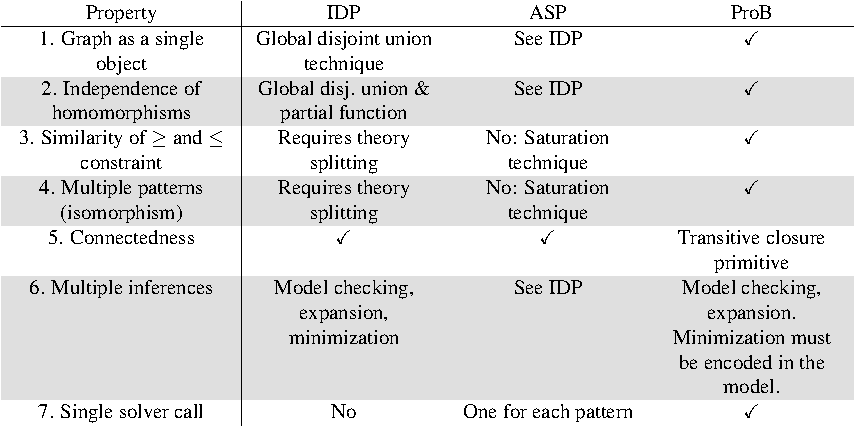
\includegraphics{PropertyTable-crop.pdf}
\end{center}
\caption{Evaluation of the desirable properties in IDP / ASP / ProB\label{tbl:conclusion}}
\end{table}

As can be seen from Table~\ref{tbl:conclusion}, 
\matthias{Provide an explanation of the table, with some references to earliers parts of the text to justify certain claims/results}


\section{Performance}\label{sec:performance}
%\matthias{This is the working ProB code that we'll show as an example}
%In this section, the graph mining problem is slightly modified: we now restrict the search for a pattern to graphs that are a subgraph of a given \emph{template} graph.
%The declarative approach allows us to implement such a modification with only minimal effort.
%\VerbatimInput{original_prob_files/PositiveAndNegative.mch}
To compare the performance of higher order and first order systems, we compared the IDP system with the ProB system (which uses higher order).
To this end, we used the positive examples of the Yoshida~\citep{yoshida_dataset} dataset, which is derived from biochemics, for graph mining.
First, we randomly picked an example to use as the template graph.
Next, we mined a pattern from this template, using the threshold value $N_{+} = 13$ (5\% of the size of the example set).
During the mining process, we tracked the time it takes to mine the $i=1..n$-th pattern. The results are averaged over ten runs.


The ProB model from Subsection \ref{subsection:prob} comes closest to the higher order formulation (as demonstrated in \textbf{Table} \ref{tbl:conclusion}), however, the solver support is not yet sufficient to efficiently execute the higher order graph mining model on larger datasets, i.e., currently we have not found an efficient way to mine patterns using a higher order B model. 
Consequently, from a KR point-of-view, we consider the higher order formulation of the graph mining problem as setting a challenge and goal for future solver techniques.
The key issue preventing an efficient higher order formulation lies in reifying the higher order existential quantifier inside the set comprehension. A possible future solution would be to provide a Prolog implementation for the homomorphism predicate (e.g., as a ProB external function).
For IDP, the results can be found in \textbf{Table} \ref{table:idp:averaged_results}.
%The results shown in \textbf{Fig.}~\ref{fig:ProBIDPComp} are the times needed to mine the $i$'th pattern, averaged over 10 repeats of the described process.
% \begin{figure}[thb]
% 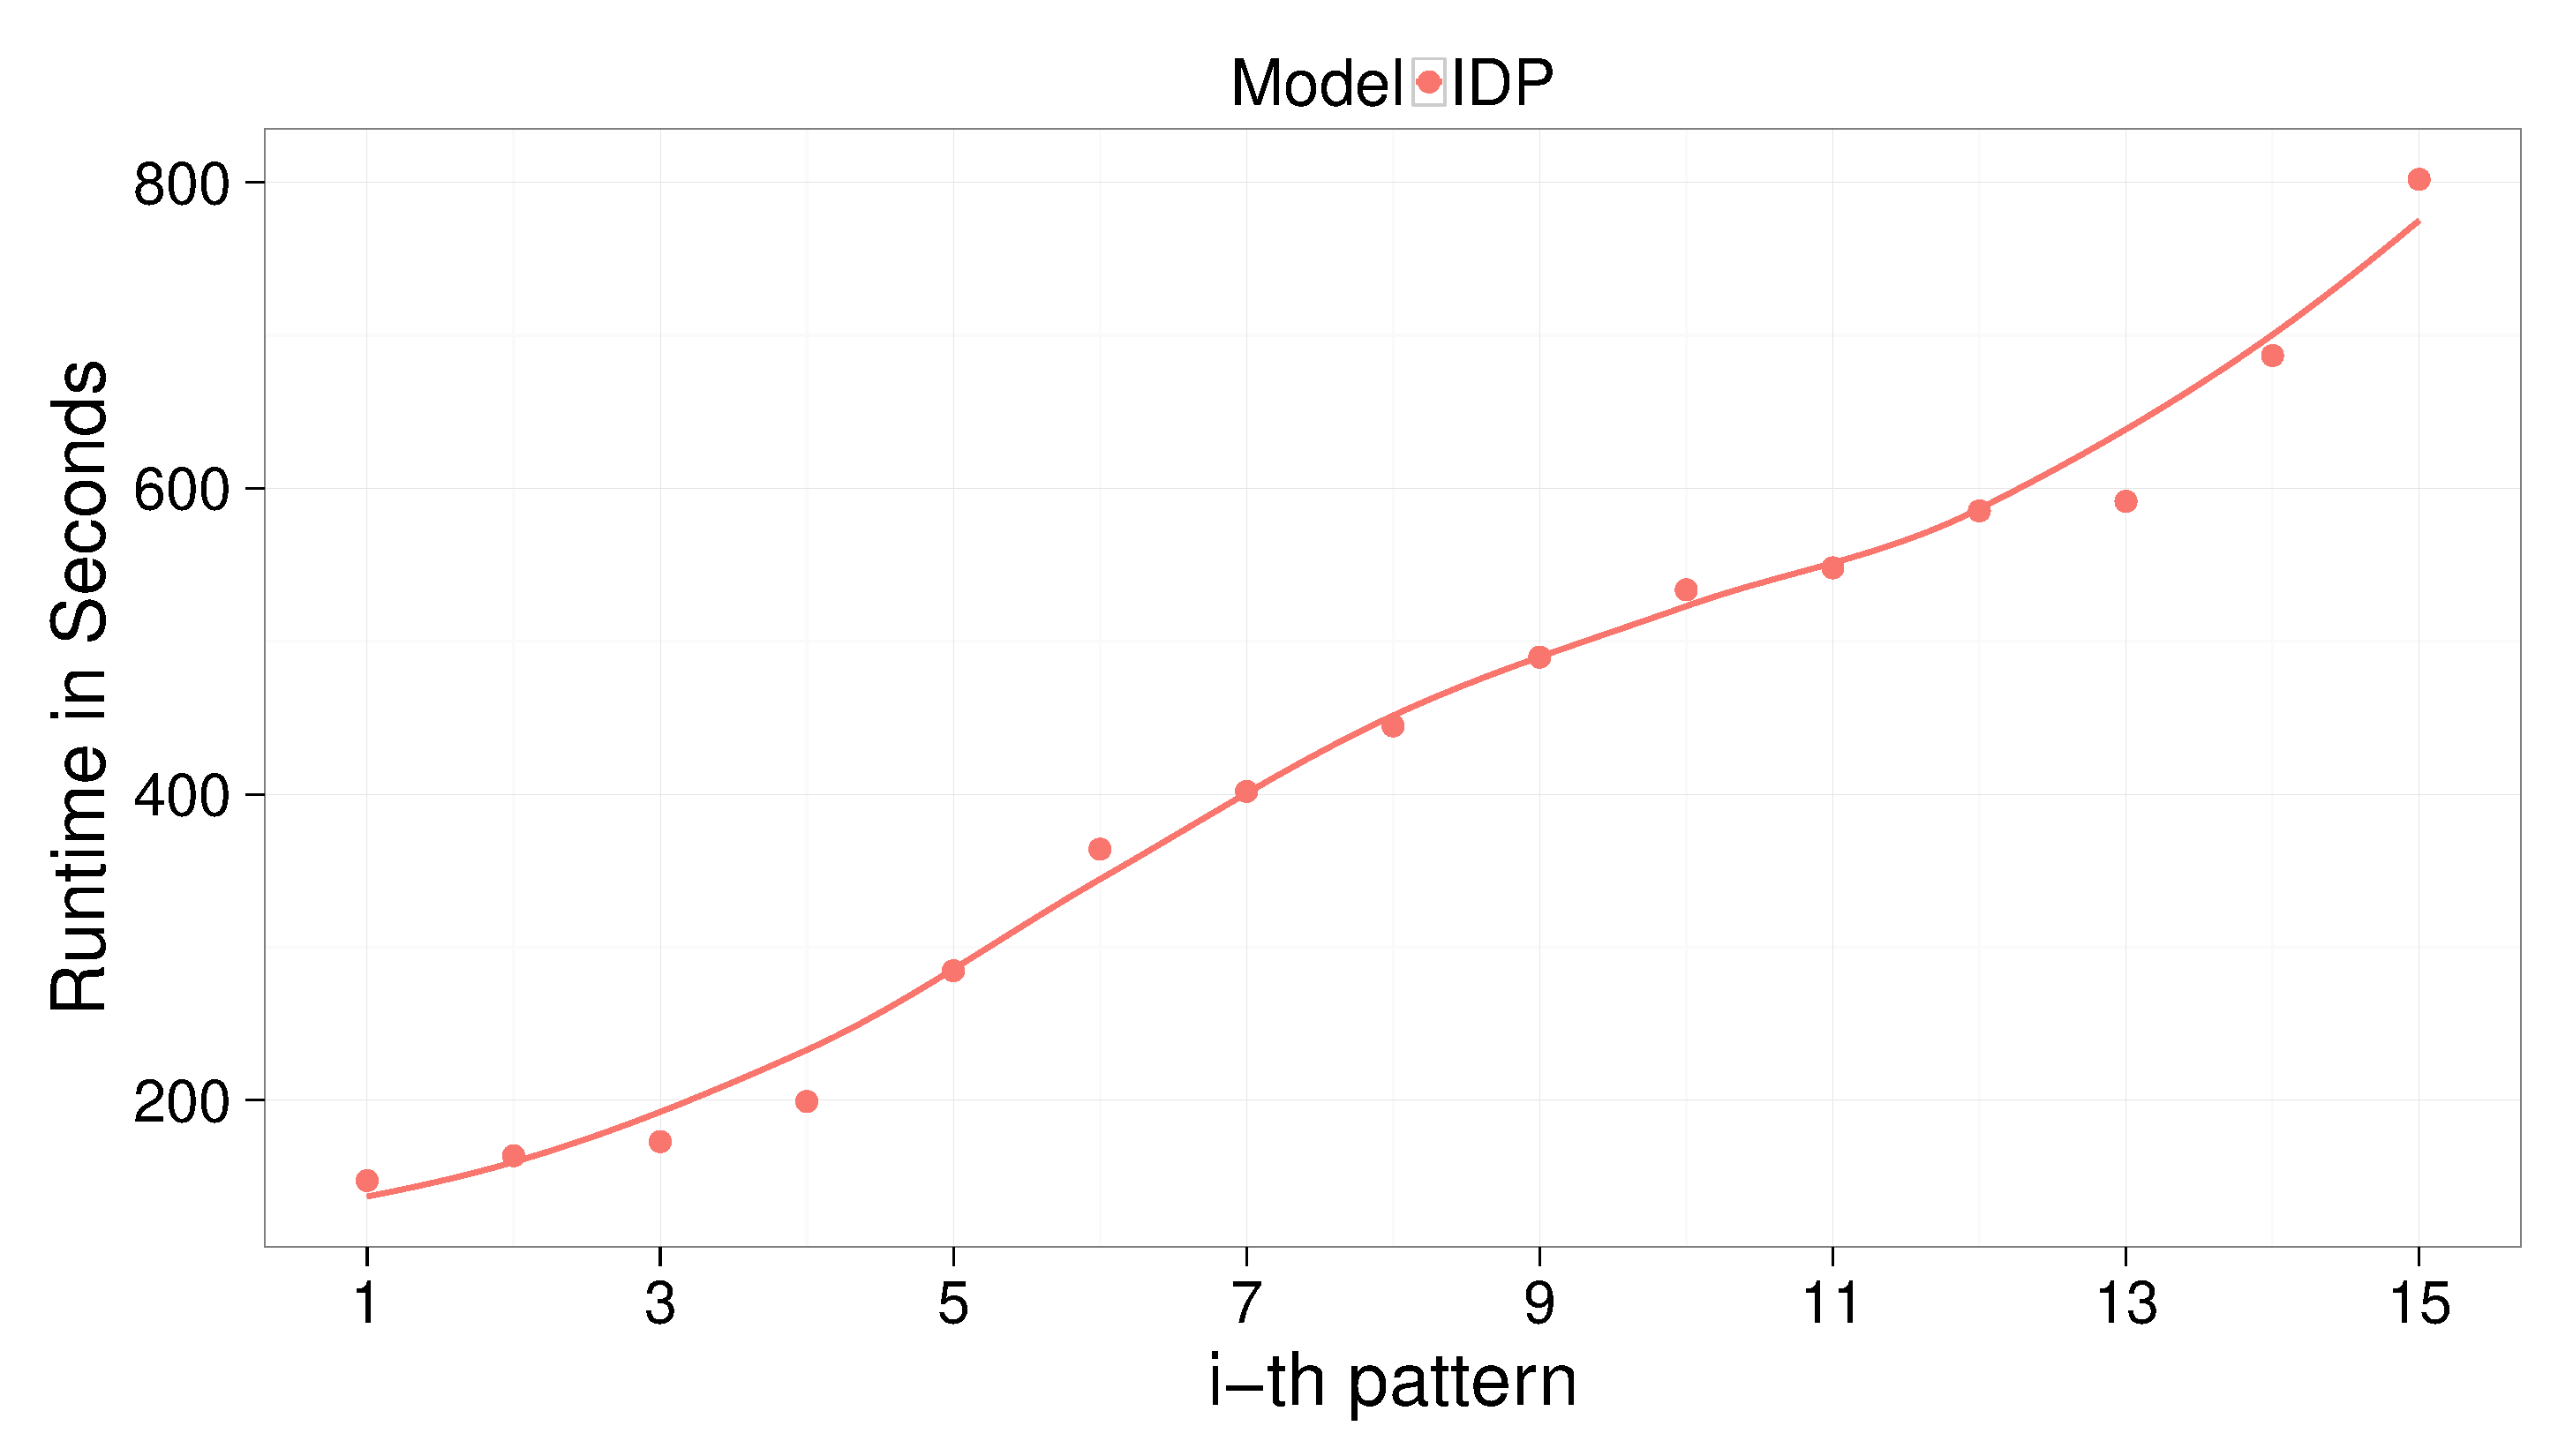
\includegraphics[scale=0.14]{extra/idp_prob_comparison.pdf}
% \caption{\footnotesize{Comparison between ProB (blue) and IDP (red) for the general graph mining problem on the Yoshida dataset} }
% \label{fig:ProBIDPComp}
% \end{figure}
% \sergey{to complete}

To analyze the effect of the disjoint union technique, we compared the performance of IDP and ASP on the Yoshida dataset using different encodings of the graph mining problem.
In \textbf{Fig.}~\ref{fig:decomposition_fol}, we see the performance of IDP (\textbf{Fig.}~\ref{fig:decomposition_idp}) and ASP (\textbf{Fig.}~\ref{fig:decomposition_asp}) on finding the $i$-th pattern.
Two different encodings are used: one that uses the disjoint union technique, and one that performs a new IDP/ASP call for every different example graph, and aggregates this data using procedural code (i.e. in a decomposed fashion).

It is clear from \textbf{Fig.}~\ref{fig:decomposition_fol} and the order(s) of magnitude difference between the decomposition and disjoint union technique that these systems can highly benefit from detecting the independence of these different subproblems and solving them separately.
We expect that expressing the problems in a higher order fashion will allow detection of this subproblem independence and allow for more performant and expressive systems.
\begin{figure}[thb]
\centering
\begin{subfigure}{.44\textwidth}
  \centering
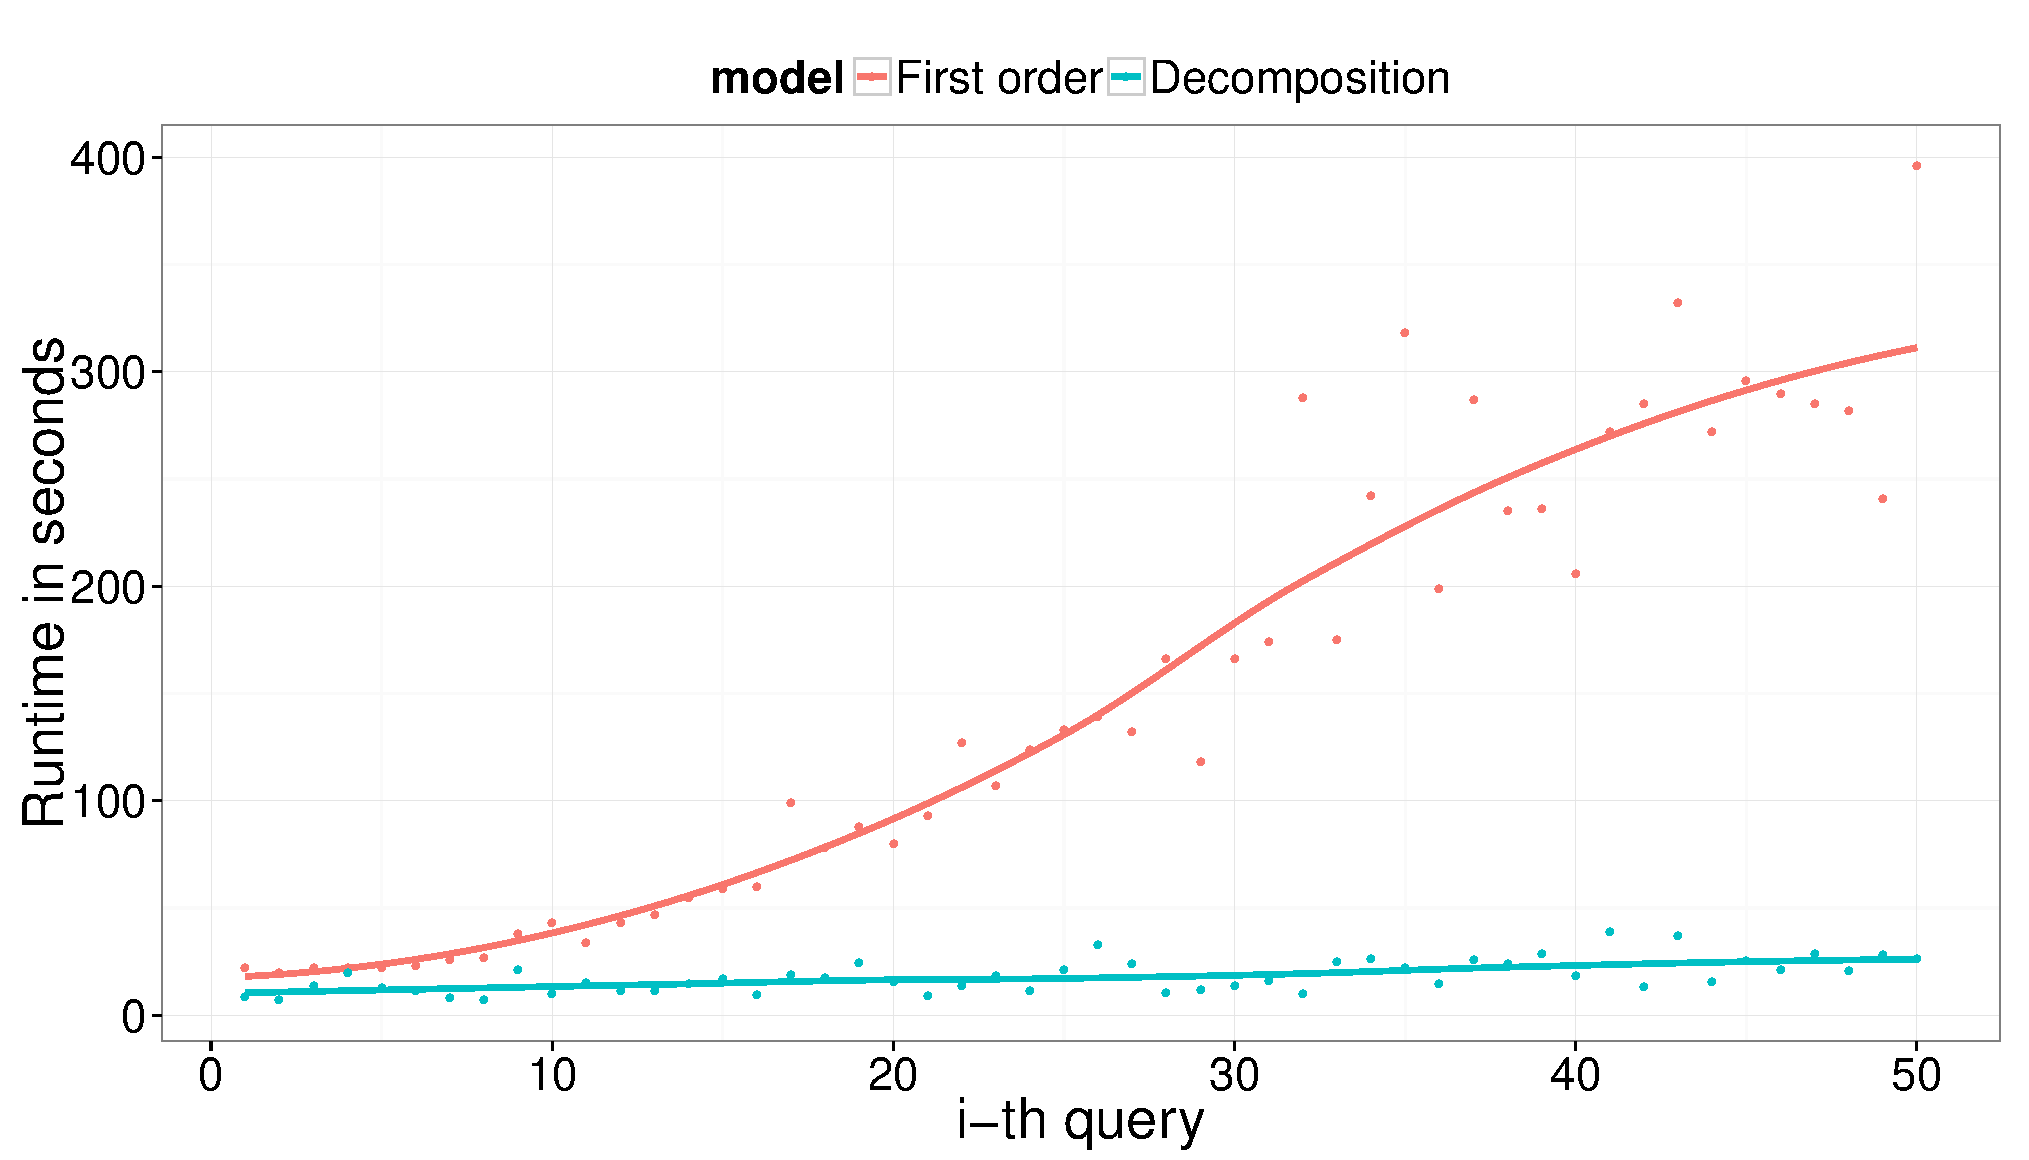
\includegraphics[scale=0.14]{extra/figure_comparison_yoshida.pdf}
\caption{\footnotesize{IDP: the disjoint model has a growing trend while the simulation stays flat. The gap is one order of magnitude. (\cite{ilp_graph_mining})}}
  \label{fig:decomposition_idp}
\end{subfigure}%
\hfill
\begin{subfigure}{0.46\textwidth}
  \centering
 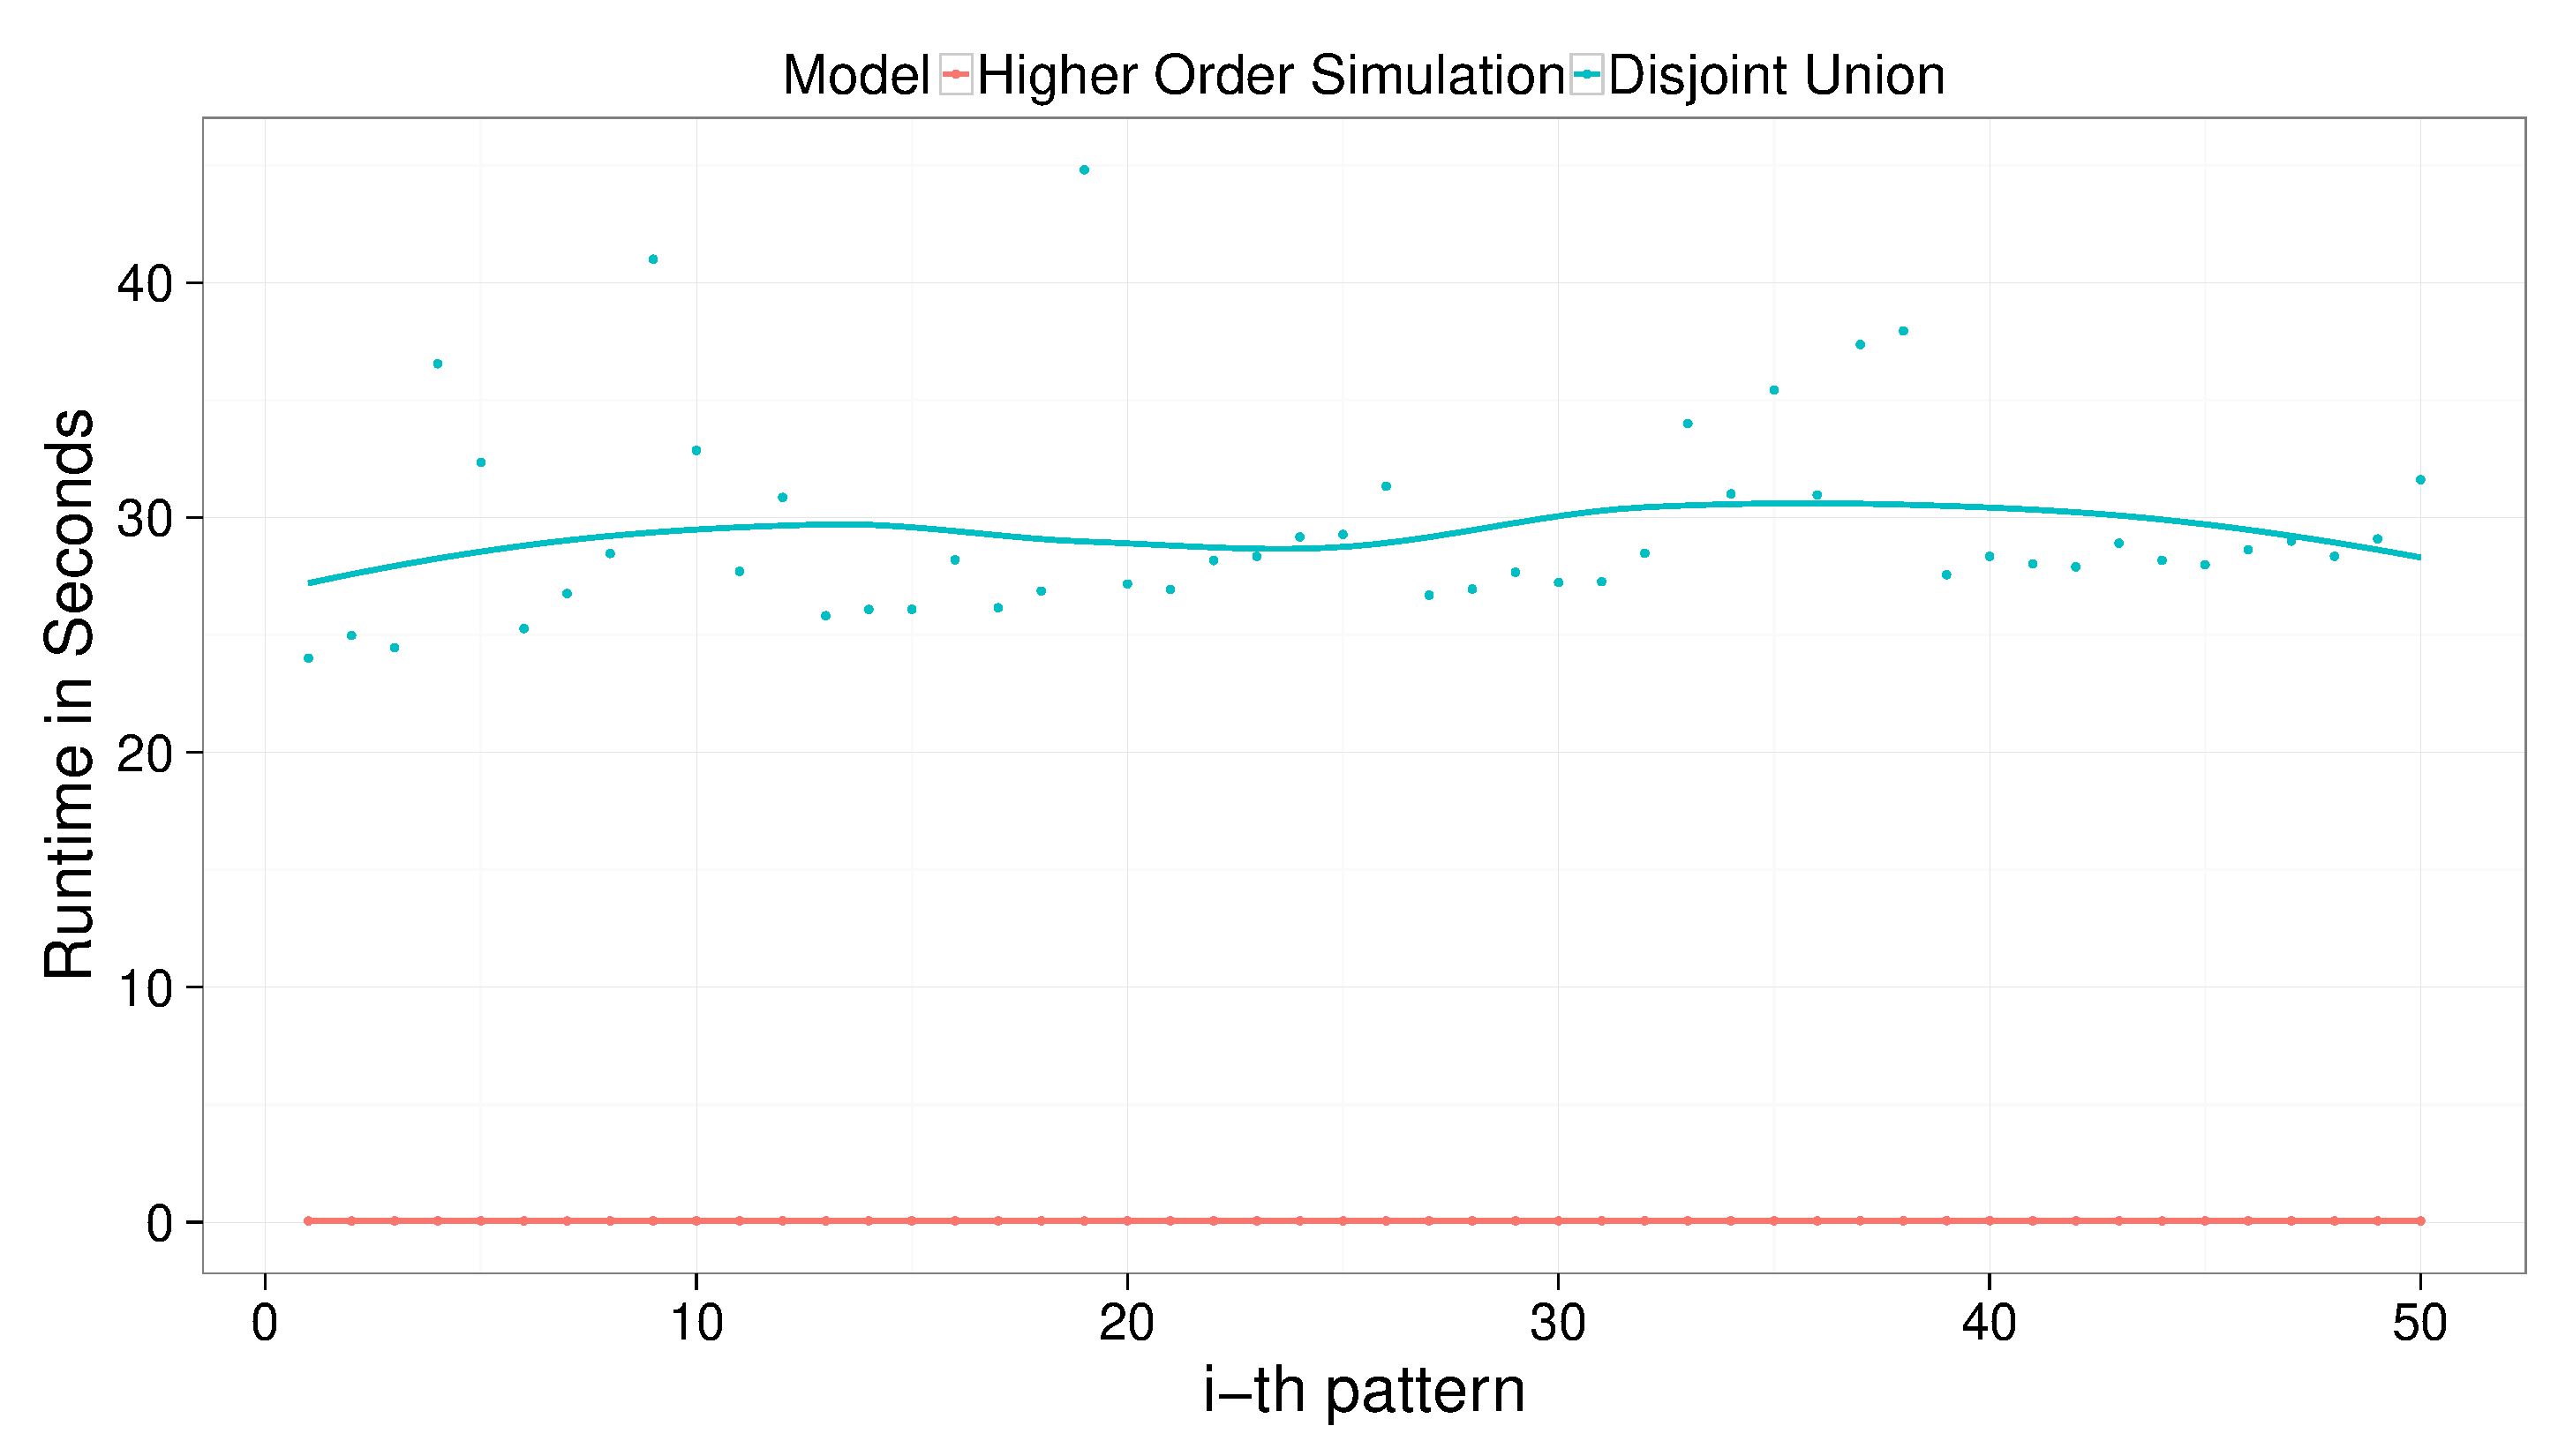
\includegraphics[scale=0.14]{extra/asp_fol_vs_decomposed_yoshida.pdf}
 \caption{\footnotesize{ASP: the disjoint model exhibits fluctuation around 30s with a slow runtime growth, while the simulation stays flat. The gap is two orders of magnitude.}}
  \label{fig:decomposition_asp}
\end{subfigure}
\caption{\footnotesize{Frequent graph enumeration problem (5\% threshold) on Yoshida dataset for IDP (a) and ASP (b), comparing disjoint union (in blue) and higher order simulations (in red). Further details can be found in \ref{sec:hol_description}.}}
\label{fig:decomposition_fol}
\end{figure}


\section{Proposed extensions}\label{sec:extension}
%\matthias{Here we will list the things we miss in each language, and introduce possible ways of implementing them and ways to learn from eachother}
\matthias{How does ProB add HO, and what can we learn from them (and vice-versa)}
In this section, we compile a list of missing language constructs, and introduce possible ways of implementing them and ways to learn from eachother.
\subsection{Language}
HO is sometimes criticized as being to expressive.
Sometimes however, the additional structure HO exhibits allows solvers to perform better.
For example, in this case HO preserves the local coherence and independence of the different examples, a property that the solver could leverage to become more efficient.
\subsection{solver}

\subsubsection{Oracles}
\subsubsection{Benders decomposition}

\subsection{Faithful encoding}
\matthias{In this subsection, we show a new encoding, which is not yet supported in IDP, and argue that it is more faithful to the problem with respect to the definition as given in Def~\ref{def:gm2}.}
\begin{lstlisting}[mathescape,style=model,caption={Faithfull encoding}]
  @\textbraceleft@
  homomorphism((Edge1, Label1), (Edge2, Label2)) $\leftarrow$
      @\big(@$\exists$ F: ($\forall$ x, y : x $\neq$ y $\implies$ F(x) $\neq$ F(y)) $\wedge$
       ($\forall$ x, y : Edge1(x, y) $\implies$ Edge2(F(x), F(y))) $\wedge$
       ($\forall$ x : Label1(x) = Label2(F(x)))@\big)@

  isomorph((Edge1, Label1),(Edge2, Label2)) $\leftarrow$
      @\big(@$\exists$ F: ($\forall$x,y:x$\neq$y$\implies$F(x)$\neq$F(y)) $\wedge$
       ($\forall$ x, y : Edge1(x, y) $\iff$ Edge2(F(x), F(y))) $\wedge$
       ($\forall$ x : Label1(x) = Label2(F(x)))@\big)@.
  @\textbraceright@

  @\textbraceleft@
  reachable(x, y, (Edge, Label)) $\leftarrow$ Edge(x, y) $\lor$ Edge(y, x).
  reachable(x, y, (Edge, Label)) $\leftarrow \exists$ : reachable(x, z, (Edge, Label)) $\wedge$ reachable(z, y, (Edge, Label)).
  @\textbraceright@
  
  isPattern(P) $\iff$
      @\big(@(@\#\textbraceleft@ Pos : positive(Pos) $\wedge$ homomorphism(P, Pos) @\textbraceright@ $\geq$ $N_{+}$) $\land$
       (@\#\textbraceleft @Neg : negative(Neg) $\wedge$ homomorphism(P, Neg) @\textbraceright@ $\leq$ $N_{-}$) $\land$
       ($\forall$ x, y : reachable(x, y, P))@\big)@.
      
  $\forall$P : pattern(P) $\implies$ isPattern(P). 
  $\forall$P,P2 : pattern(P)$\wedge$pattern(P2)$\wedge$P$\neq$P2 $\implies$ $\neg$isomorph(P, P2).

\end{lstlisting}


This encoding compactly specifies the graph mining problem, in a way that closely corresponds to its mathematical definition.
To allow inferences on this theory, extended solver support is necessary.
We now identify possible ways in which a solver can provide this additional support:

\subsubsection{Data representation}

One possible way to solve these higher order theories is based on the disjoint union technique: 
We automatically derive a \emph{disjoint union} specification from this higher order theory.
By analyzing the different rules in the specification, the solver can derive that the only \matthias{one of the? (zie later)} higher order objects consist of an edge relation and a labeling function.
It can then introduce these relations automatically, indexed by an identifier.
Quantifications over these higher order objects become quantifications over these identifiers.
\matthias{Furthermore the solver must also detect the existential quantification of the function $f$.
This too leads to a disjoint union }

Another way is to automatically introduce separate predicates and functions for each higher order object. 
The solver subsequently replicates the necessary rules specified for these separate predicates and functions. \matthias{Dit gaat eigenlijk alleen in combinatie met de subsolver approach, omdat ik in het geval van een universele quantificatie over een predicaat waar gezocht wordt niet weet hoeveel keer ik de regels moet instantiëren.}

\subsubsection{Negative contexts}
First, the solver must detect existential higher order quantifications.
When an existential quantification occurs in a negative context, 

\matthias{Wanneer je (lokaal) herschrijft naar ESO komen al je coNP problemen (die je zéker in een subsolver moet steken) voor in negatieve context. Ik dacht dus ook dit apart te behandelen van de data representatie. Hier moet echter de kanttekening van boven bij gemaakt worden dat alleen in dit geval de replication methode haalbaar lijkt...}
%% !TEX root = notes.tex
\section{Related Work}\label{sec:related_work}
There is a number of research directions related to our work. We group them by what they have in common with our work and contrast the difference with each group.

\paragraph{Declarative Pattern Mining} There has been a lot of work on declarative pattern mining for unstructured data focused on: \textit{itemset mining} in the context of constraint programming \citep{tias_original,mining_cp_extra,tias_declarative_pattern_mining}, as well as in ASP \citep{asp_itemset} and SAT \citep{itemset_sat}, and \textit{tiling} in the context of ASP \citep{relational_decomposition} and of CP \citep{ranked_tiling}. 

Recently people started looking at the structured declarative pattern mining such as \textit{sequence mining} in CP \citep{cp_sequence_mining} and ASP \citep{rennes_asp_sequences}, and \textit{graph mining} in IDP \citep{ilp_graph_mining}. \sergey{I hope by this time IDP is very well explained and introduced, so I can just leave it as ``it is''} The main focus of these works is on the encoding techniques that allows one to encode model using existing language concepts and primitives, i.e., on the coding and execution but not on the model and language itself. From the KR point view, the latter work on graph mining is of a preliminary character, since it does not provide a deep knowledge representation analysis of the model with respect to the mismatch between higher order logical model and the executed model. Neither the most interesting practical case of discriminative mining was not investigated in detail, nor any comparison between ASP, IDP and ProB was provided. \sergey{Should it be phrased less harsh here?}

\citet{declarative_structured_language} proposed a generic framework that relies on the concept of \textit{operators} as building blocks of structured pattern mining. The key difference is in the design of the framework, it is inspired by the specialized algorithms and supposed to mimic their search techniques. Theoretically, the framework we have proposed in this paper can benefit from the ideas of operators and the search techniques described in the former, e.g., we can design a solver that would call a logical engine in a certain order keeping the context of the previous computations and therefore mimic the behaviour of the specialized algorithms, nevertheless using declarative specification for the operators.

\sergey{explain that higher order problem already occurs here}

\paragraph{Graph Mining} A number of classic algorithms has been developed over the years. They are designed to solve only particular topic and typically require complete rewriting of the algorithm to solve a new variation of the problem. For example the key component of structured mining \textit{the matching operator} exists in many versions: mining under homomorphism \citep{theta_subsumption} and under subgraph isomorphism \citep{gspan} for the general case of graphs, and for the subclass of trees there are three other matching operators \citep{subtree_overview}. Also the algorithms need to be adapted for the presence of various constraints, e.g., algorithms need to be changed to handle discriminative setting that is known to be particularly useful in applications \citep{pattern_mining_classification}

\paragraph{Graph Modeling} An interesting approach within CP paradigm is to to a domain specific primitives to the language. In the domain of graph combinatorial problems, there is a work in that directions called CP(graph) \citep{cp_graph}, where graph related primitives are integrated into the language: graph variables and certain types of graph constraints are supported. It is not however designed for mining problems and therefore does not discuss constraints for canonicity or matching. It is designed for only particular domain of graphs and it is unclear how to generalize it to our setting and other relational mining tasks.
% !TEX root = notes.tex
\section{Conclusion and future work}\label{sec:conclusion}
\matthias{A conclusion}



{\scriptsize
\bibliography{references}}
\bibliographystyle{abbrvnat}
\setcitestyle{authoryear,open={(},close={)}}

\newpage
\appendix
\section{Code}
\label{app:Code}
This appendix provides the relevant code for the IDP, ASP and ProB systems.
The full IDP code is available at \url{}, while the ASP code is available at \url{} and the ProB code at \url{}. \todo{Sergey: Provide these urls!} 
\begin{lstlisting}[caption=IDP positive constraint, style=model, label=lst:IDPPos]
vocabulary V{
  type node isa nat
  type graphid
  type label

  // Predicates determining the template graph.
  template_edge(node, node) 
  template_label(node):label

  // Predicates describing the positive example graphs
  example_edge(graphid, node, node)
  label(graphid, node):label
  threshold: int

  // Predicates describing the pattern graph
  inpattern(node) // True for the nodes which occur in the pattern
  partial f(graphid, node):node // Represents the homomorphisms with the example graphs
  homowith(graphid) // True for graphs for which f represents a correct homomorphism
  path(node, node) // path(a,b): True if there exists a path from a to b in the pattern
}

theory Positive:V_Pos{
   //The pattern is a connected subgraph of the template: From every node in the pattern, 
   //there exists a path to every other node in the pattern.
   !x,y[node] : x ~= y & inpattern(x) & inpattern(y) => path(x,y).
   {
      path(x,y) <- template_edge(x,y) & inpattern(x) & inpattern(y).
      path(x,y) <- ?z[node] : path(x,z) & path(z,y).
      path(x,y) <- path(y,x).
   }

   //existence of a homomorphic f from the pattern to example graph with graphid gid.
   !gid[graphid] : !x[node]   : homowith(gid) & inpattern(x) <=> ? y[node] : y=f(gid,x).
   !gid[graphid] : !x,y[node] : homowith(gid) & inpattern(x) & inpattern(y) & x~=y => f(gid, x) ~= f(gid,y).
   !gid[graphid] : !x,y[node] : homowith(gid) & inpattern(x) & inpattern(y) & template_edge(x,y) => edge(gid, f(gid,x). f(gid,y)).
   !gid[graphid] : !x[node] : homowith(gid) & inpattern(x) => template_label(x) = label(gid, f(gid,x)).

   // At least N homomorphisms must be found
   #{ gid [graphid] : homowith(graph) } >= threshold.
}
\end{lstlisting}


\lstset{basicstyle=\footnotesize\ttfamily,breaklines=true}
\begin{lstlisting}[caption=ASP positive matching, style=model]
homowith(G) | not_homowith(G) :- positive(G).

1 { f(G,X,V) : node(G,V) } 1 :- positive(G), inpattern(X).

:- homo_with(G), f(G,X,V1), f(G,Y,V2), template_edge(X,Y), 
not edge(G,V1,V2), inpattern(X), inpattern(Y).

positive_count(N) :- N = #count{G:homowith(G)}.

:- positive_count(N), N < 2.
\end{lstlisting}

\begin{lstlisting}[caption=ASP negative matching using saturation technique, label={lst:aspsaturation}, style=model, numbers=left]
map(G,X,v1) | map(G,X,v2) | map(G,X,v3) | map(G,X,v4) :- invar(X), negative(G). @\label{lstline:probspec}@
map(G,X,V) :- saturated(G), t_node(X), node(G,V).

saturated(G) :- t_edge(X,Y), map(G,X,V1), map(G,Y,V2), not edge(G,V1,V2), negative(G), invar(X), invar(Y).
saturated(G) :- map(G,X,V),  map(G,Y,V), X != Y, invar(X), invar(Y). // we cannot map two different template nodes to the same 

neg_homowith(G) :- not saturated(G), negative(G).

negative_count(N) :- N = #count{G:neg_homowith(G)}.
:- negative_count(N), N > 1.

\end{lstlisting}

\begin{lstlisting}[caption=Canonicity template-based check, style=model]
iso(X,x1) | iso(X,x2) | iso(X,x3) | iso(X,x4) :- invar(X).

candidate_var(X) :- iso(_,X).

%not iso!
iso_saturated :- invar(X1), invar(X2), iso(X1,V1), iso(X2,V2),     t_edge(V1,V2), not t_edge(X1,X2). 
iso_saturated :- invar(X1), invar(X2), iso(X1,V1), iso(X2,V2), not t_edge(V1,V2),     t_edge(X1,X2).

iso(X,V) :- invar(X), t_node(V), iso_saturated.

d1(X) :-     invar(X), not candidate_var(X). 
d2(X) :- not invar(X),     candidate_var(X).

not_equal :- d1(X). % check that in fact candidate is different from the pattern itself
not_equal :- d2(X). % check that in fact candidate is different from the pattern itself

iso_saturated :- not not_equal. % should not be completely equal

min_d1(N) :- N = #min{ X: d1(X) }, not iso_saturated.
min_d2(N) :- N = #min{ X: d2(X) }, not iso_saturated.

iso_saturated :- min_d1(N1), min_d2(N2), N1 > N2.
\end{lstlisting}

\begin{lstlisting}[caption=Auxilary predicates -- probably should be moved to appendix, style=model]
%selects subpattern

t_path(X,Y) :- t_edge(X,Y), invar(X), invar(Y).
t_path(X,Y) :- t_edge(X,Z), t_path(Z,Y), invar(X).

:- invar(X), invar(Y), not t_path(X,Y).

0 { invar(X) } 1 :- t_node(X).
% auxilary constraints


edge(G,Y,X) :- edge(G,X,Y).
t_edge(Y,X) :- t_edge(X,Y).
node(G,Y)   :- edge(G,Y,_).
t_node(X)   :- t_edge(X,_).
\end{lstlisting}

\begin{lstlisting}[caption=Canonicity previous solution isomorphism check, style=model]
iso(s1,X,x1) | iso(s1,X,x2) :- invar(X).
iso(s2,X,x2) | iso(s2,X,x3) :- invar(X).

candidate_var(G,X) :- iso(G,_,X).

iso_saturated(G) :- invar(X1), invar(X2), iso(G,X1,V1), iso(G,X2,V2),     t_edge(V1,V2), not t_edge(X1,X2). 
iso_saturated(G) :- invar(X1), invar(X2), iso(G,X1,V1), iso(G,X2,V2), not t_edge(V1,V2),     t_edge(X1,X2). 
iso_saturatea(G) :- not equal(G), iso(G,_,_). 

iso(G,X,V) :- invar(X), t_node(V), iso_saturated(G).

:- not iso_saturated(G), iso(G,_,_).

d1(G,X) :-     invar(X), not candidate_var(G,X), iso(G,_,_).
d2(G,X) :- not invar(X),     candidate_var(G,X).

not_equal(G) :- d1(G,X). % check that in fact candidate is different from the pattern itself
not_equal(G) :- d2(G,X). % check that in fact candidate is different from the pattern itself

equal(G) :- not not_equal(G), iso(G,_,_).

\end{lstlisting}

\end{document}
